\documentclass[useAMS,usenatbib]{mn2e} 
\usepackage{graphicx}
\usepackage{amsmath}
\usepackage{amssymb}
\usepackage[font={it},labelfont={bf}]{caption}
\usepackage{units}
\usepackage{times}
\usepackage{color}
\usepackage[usenames,dvipsnames,svgnames,table]{xcolor}

\usepackage{fixltx2e} % fixes placing of image positions

\definecolor{customhdrcolor}{rgb}{0.0,0.0,0.0}
%\definecolor{customcitecolor}{rgb}{0.0,0.25,0.25}
\definecolor{customcitecolor}{rgb}{0.0,0.5,0.75}
%\definecolor{customlinkcolor}{rgb}{0.0,0.0,1.0}
\definecolor{customlinkcolor}{rgb}{0.0,0.5,0.75}

\usepackage[colorlinks=true,linkcolor=customlinkcolor,urlcolor=customlinkcolor,citecolor=customcitecolor,pdftex]{hyperref}

\ifpdf\pdfinfo{/Title      (The brightness and spatial distributions of terrestrial radio sources)
               /Author     (A. R. Offringa et al.)
               /Keywords   (dark ages, reionization, first stars;atmospheric effects;instrumentation: interferometers;methods: observational;techniques: interferometric;radio continuum: general;rfi)
        }
\else\usepackage{graphics}\fi

\setlength{\pdfpageheight}{\paperheight}
\setlength{\pdfpagewidth}{\paperwidth}


\title[Brightness and spatial distributions of terrestrial radio sources]{The brightness and spatial distributions of terrestrial radio sources}

\author[A.~R.~Offringa et al.]{
  A.~R.~Offringa$^{1,2}$\thanks{E-mail:
\url{offringa@mso.anu.edu.au}},
  A.~G.~de~Bruyn$^{2,3}$,
   and S.~Zaroubi$^{2}$\\
$^{1}$Australian National University, RSAA Mt. Stromlo Observatory, Cotter Road, Weston Creek ACT 2611, Australia\\
$^{2}$University of Groningen, Kapteyn Astronomical Institute, PO Box 800, 9700 AV Groningen, The Netherlands\\
$^{3}$ASTRON, PO Box 2, 7990 AA Dwingeloo, The Netherlands
}

\begin{document}

\date{Accepted [TODO date]. Received [TODO date]; in original form [TODO date]}
\pagerange{\pageref{firstpage}--\pageref{lastpage}}
\pubyear{2012}

\maketitle
\label{firstpage}

\begin{abstract}
Feeble undetected sources of radio-frequency interference (RFI) might become visible after integration of long radio observations if they are coherently present over time. Thereby, they might obstruct the detection of the astronomical signal of interest. This issue is especially important for Epoch of Reionization (EoR) projects that try to detect the faint redshifted HI signals of the earliest objects in the Universe. We explore the low-frequency RFI situation by studying the $\log N$--$\log S$ histograms of data observed with LOFAR. The histograms shows an RFI distribution that follows a power-law distribution with an estimated exponent around -1.6 to -1.5. With several assumptions, this can be explained with a uniform distribution of terrestrial radio sources whose radiation follows existing propagation models. Extrapolation of the power law would imply that the current LOFAR EoR observations should be severely RFI limited if these sources are coherently present. Since these observations have achieved the thermal (sky) noise limit, a logical implication is that most of the RFI sources do not add coherently.
\end{abstract}

\begin{keywords}
atmospheric effects -- instrumentation: interferometers -- methods: observational -- techniques: interferometric -- radio continuum: general -- dark ages, reionization, first stars
\end{keywords}

\section{Introduction}
Radio astronomy concerns itself with the observation of radiation from celestial sources at radio wavelengths. However, astronomical radio observations can be affected by radio-frequency interference (RFI), which makes it difficult to calibrate the instrument and achieve high sensitivities \citep{impact-of-warc79,interference-and-radioastronomy-1991,interference-model-lemmon,rfi-mitigation-overview-fridman-baan}. Many techniques have been designed to mitigate this effect, such as detection and flagging of data \citep{chi-square-time-blanking-weber, multichannel-rfi-mitigation, exoplanet-detection-with-rfi, wsrt-rfims, pulse-blanking, effelsberg-rfi-mitigation, LOFAR-RFI-pipeline}, adaptive cancellation techniques \citep{adaptive-cancellation,post-correlation-reference-signal} and spatial filtering \citep{multichannel-rfi-mitigation, ellingson-spatial-nulling-2002, hampson-spatial-nulling-2002, boonstra-dissertation, spatial-filtering-parkes-multibeam-for-pulses, post-correlation-filtering}. In most cases, these methods excise enough of the interference to calibrate and image the data.

Typical radio observations record a few hours of data, and the results are integrated. In these cases, it often suffices to only excise interference that is apparent and thus above the noise to reach the thermal noise limit of the instrument. A new challenge arises, however, when one desires much deeper observations, and hundreds of hours of observations need to be integrated. In such a case, feeble interference caused by stationary sources might not manifest itself above the noise in individual observations, but is coherently present in the data. Subsequently, when averaging these data, the interference might become apparent and occlude the signal of interest. This is very relevant for the 21-cm Epoch of Reionisation (EoR) experiments, because they involve long integration times. Several such experiments are underway, to either measure the angular power spectrum \citep{gmrt-eor-2011-paciga,de-bruyn-eor-ursi-2011,eor-paper-2011-jacobs,eor-mwa-2012-williams} or the global signal \citep{edges}. For these experiments, it is important to know the possible effect of low-level interferences on the data, as these might overshadow or alter the signal of interest. In this article, we will connect new insights about RFI to the angular Epoch of Reionisation experiment that is using the Low-Frequency Array \citep{de-bruyn-eor-ursi-2011}.

This work explores the information that is present in interference distributions, in order to analyse possible low-level interference that is not detectable by standard detection methods. Our approach is similar to the radio source count analysis that is used in cosmology \citep{vonhoerner-radio-source-counts}, also named $\log N$ -- $\log S$ analysis, where $N$ and $S$ refer to the celestial source count and brightness respectively. The slope in such a plot contains information about source populations, their luminosity functions and the geometry of the Universe. We analyse such a double-logarithmic plot for the case of terrestrial sources, with the ultimate goal of predicting their full spatial and brightness distributions. This results in a better insight in the effects of low-level interference and allows one to simulate the effects of interference more accurately. A distribution can be expressed either as a differential or cumulative function. This work uses differential distributions, because they are better suited for visualizing the parameters we are interested in, although the two basically convey the same information.

%TODO maybe also discuss atmospheric (lightning), e.g. see 'Harry M. Hall, A New Model for ``Impulsive'' phenomena: application to atmospheric-noise communication channels', as contains also discussion on energy distributions.

This paper is organised as follows: in Sect.~\ref{sec:distribution-prediction}, we predict the terrestrial interfering source distribution based on various assumptions. Sect.~\ref{sec:distribution-methods} presents the methods that we use to generate and analyse the histograms. This is followed in Sect.~\ref{sec:dist-data} by a short description of the two LOFAR data sets that have been used to perform the experiment. The results of analysing the sets are presented in Sect.~\ref{sec:dist-results}. Finally, in Sect.~\ref{sec:dist-discussion} the results are discussed and conclusions are drawn.

\section{Predicting the brightness distribution} \label{sec:distribution-prediction}
Interference is generated by many different kind of transmitters, and these will have different spatial and brightness distributions (``spatial'' refers here to the distribution on the Earth). For example, aeroplanes and satellites have widely different heights, while other sources are ground-based. Even ground-based sources might be spread differently. For example, it can be expected that citizens' band (CB) devices, that are often used in cars, are differently distributed from broadcasting transmitters. The frequencies of deliberately transmitting sources of a particular class of devices are constrained by the bands that have been allocated for the given class, which might allow one to distinguish different sources to some extent.

In a time-frequency plot, interfering sources can have complex structures. They can also be intermittent and different sources might overlap in time-frequency space. An example of interfering sources can be seen in Fig.~\ref{fig:dist-rfi-example}, which shows raw visibility data of one baseline of a LOFAR observation in a time-frequency diagram (dynamic spectrum). Because many sources change over time, are repetitive or affect multiple channels, many sources produce multiple unconnected features in the time-frequency diagram. It is often not clear what constitutes a single interfering source, hence it is hard to count individual sources. Instead, we will count the number of times a given brightness occurs in time-frequency space. This --- as well as many other effects --- will of course influence the distribution. First we will derive the expected intrinsic source distribution. After that, we will analyse the issues that arise when measuring the distribution by counting samples.

\begin{figure*}
\begin{center}
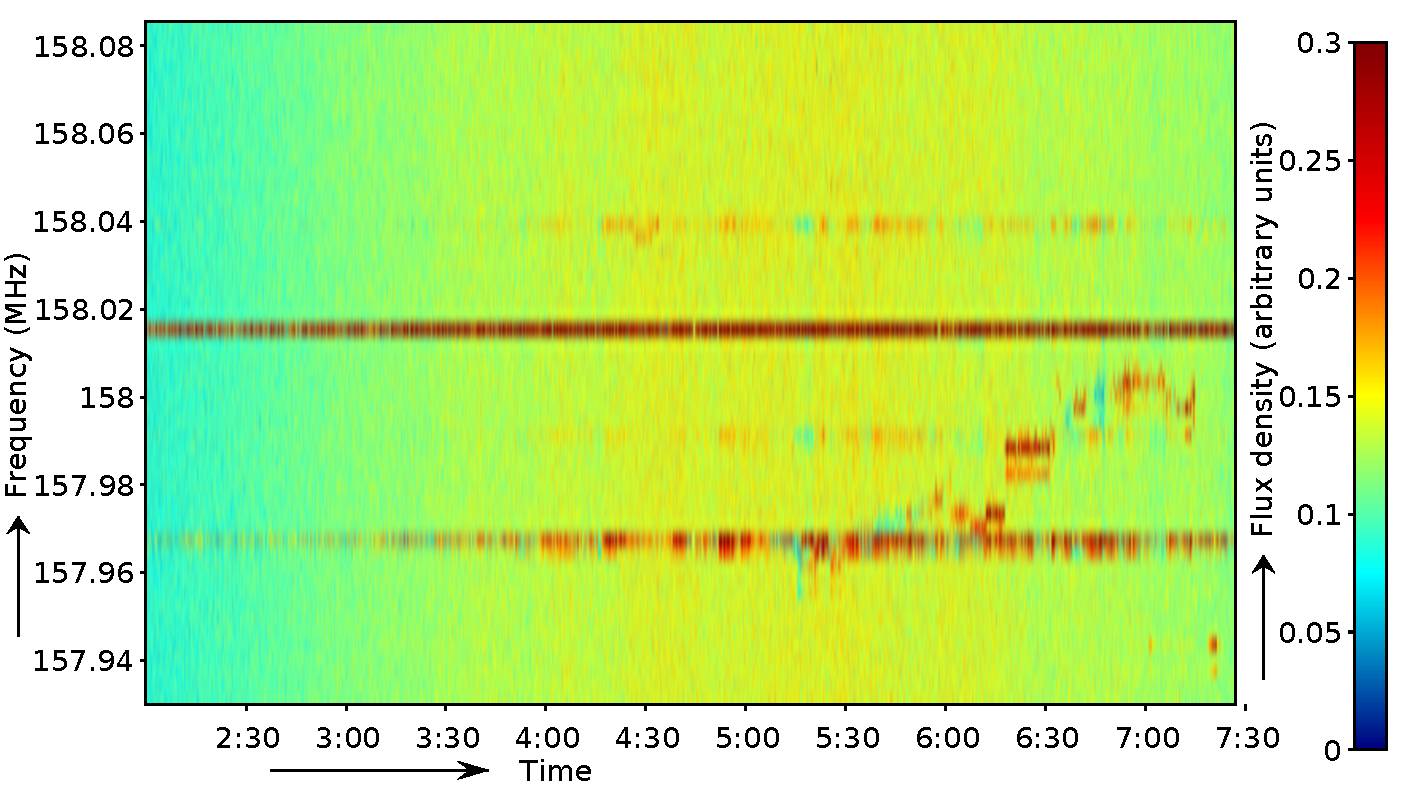
\includegraphics[height=8cm]{img/TF-L43786_L220-rfi-example.pdf}
\caption{A small part of an observation displayed in a time-frequency plot. The features with significantly higher values are caused by interference. Some of these have a constant frequency, while others are more erratic.}
\label{fig:dist-rfi-example}
\end{center}
\end{figure*}

In every dynamic spectrum we can measure the number of times that the flux density is within a particular range. Dividing this quantity by the total number of samples yields the relative number of events as a function of intensity. We will refer to this quantity with the statistical term ``frequency density'' (not to be confused with the physical radiation frequency). We will now start by deriving a prediction of the frequency density function of ground-based interfering sources. Consider an interfering point source of strength $I$. This source is observed by an interferometer that consists of two antennae or stations with gains $g_1,g_2$, which include all instrumental effects. The antennae are located at distances $r_1,r_2$ from the source. The interferometer will record an apparent instantaneous strength $\mathcal{S}$ of
\begin{equation}
 \mathcal{S}(r_1, r_2) = I \frac{g_1 g_2}{r_1 r_2},
\end{equation}
with $g_1,g_2>0$ and $r_\textrm{L} > r_1,r_2 > 0$. Here, $r_\textrm{L}$ is a limiting distance, which will be well below the diameter of the Earth. We will limit our analysis to cross-correlated antennae; the auto-correlations will be ignored.

We assume that the source observed is fully coherent, but a possible decoherence factor can be absorbed in the gains. Due to the small bandwidth of most interfering sources, most RFI will be received coherently, because of the narrow-band condition. For example, if the bandwidth of the signal $\Delta\nu=1$ kHz, the narrow-band condition $\Delta \nu \ll (2\pi \tau)^{-1}$ with correlation delay $\tau$ will hold for baselines up to a few km, because it holds as long as the baseline length is significantly less than $\Delta x = c / (2 \pi \Delta \nu) \approx$ 50 km.

Now, we can treat the interferometer geometrically as a single point, as both antennae will see the same distribution. Then, we can express the received amplitude $\mathcal{S}$ for a given distance $r$ and gain $g$ as
\begin{equation} \label{eq:amplitude-fall-off-in-free-space}
 S(r) = \frac{Ig}{r^2}.
\end{equation}

Next, we assume that all sources have equal constant strength $I$ and follow a uniform spatial distribution in a two-dimensional plane. This is obviously a simplification, as the sources are actually distributed on the surface of a sphere. Hence, beyond some distance, the Earth will partly block the path between transmitter and receiver. Therefore, the assumption of uniformly distributed sources on a two-dimensional plane is only approximately valid. Using these assumptions, we can express the expected cumulative frequency density of sources $f_I(r)$ at distance $r$ as
\begin{equation} \label{eq:cumulative-distance-function}
F_{\textrm{distance} \le r}(r)=c\pi r^2,
\end{equation}
for some constant $c$ that represents the number of sources per unit area. In other words, we will observe $F$ sources that are at most a distance of $r$ away.

We need the reverse of Eq.~\eqref{eq:cumulative-distance-function} to predict the amplitude distribution, because sources with an amplitude of \emph{at most} a given strength will have a distance of \emph{at least} some distance. Sources with at least a distance of $r$ are given by $F_{\textrm{distance} \ge r}(r) = N - c\pi r^2$, with $N$ the total number of sources.

The cumulative number of sources $F_{\textrm{amplitude} \le S}$ that have an amplitude of at most $S$ can now be calculated with
\begin{align} \label{eq:cumulative-rfi-distribution}
 F_{\textrm{amplitude} \le S}(S) = & F_{\textrm{distance} \ge r}(\mathcal{S}^{-1}(r))\\
\notag = & F_{\textrm{distance} \ge r}(\pm\sqrt\frac{Ig}{S})\\
\notag = & N-\frac{c\pi Ig}{S}
\end{align}
where $\mathcal{S}^{-1}$ is the inverse of $\mathcal{S}(r)$, i.e., the function that returns the distance $r$ for a given amplitude $S$. Finally, the differential frequency density can be calculated by taking the derivative,
\begin{align} \label{eq:two-dimensional-distribution}
 f_S(S) = & \frac{dF_{\textrm{amplitude} \le S}}{dS} = \frac{c\pi Ig}{S^2}.
\end{align}

Therefore, if we plot the histogram of the RFI amplitudes in a $\log$-$\log$ plot, we predict to see a slope of $-2$ over the interval in which the RFI sources are spread like uniform sources on a two-dimensional plane. Therefore, RFI follows a power-law distribution.

\subsection{Spherical case}
If we do take into account the fact that the sources lie on a sphere instead of a plane, Eq.~\eqref{eq:cumulative-distance-function} changes. In this case, the number of sources corresponds with the surface area of a hemisphere. By using the formula for the surface area of a hemisphere and some basic geometry, one finds that
\begin{equation}\label{eq:cumulative-spherical}
\tilde{F}_{\textrm{distance} \le r} = c 2\pi R^2\left(1-\cos(2\arcsin \frac{r}{2R})\right) \hspace{0.4cm}\textrm{with } r \le 2R,
\end{equation}
with $R$ the radius of the Earth. Eqs.~\eqref{eq:cumulative-distance-function} and \eqref{eq:cumulative-spherical} have the same value over the range they can be evaluated. Therefore, the spherical and 2-dimensional cases lead to a distribution with equal power law. Evaluating Eq.~\eqref{eq:cumulative-spherical} is limited to $r \le 2R$, but in practice the lowest amplitude of observed sources is further constrained because of the curvature of the Earth. This causes distant sources to settle below the horizon. Nevertheless, some of those sources might still be visible due to reflection of the ionosphere and other (semi-)spherical propagation effects.

\subsection{Propagation effects}
So far, we have assumed that the electromagnetic radiation propagates through free space, resulting in a $r^{-2}$ fall-off. In reality, the radiation will be affected by complicated propagational effects. Because of the irregular surface of the Earth (including urban areas) and the absence of a direct line of sight between transmitter and receiver, the propagation mode might be indirect. Multiple indirect paths might be formed by reflection, refraction or diffraction of the electromagnetic wave. 

A commonly used propagation model is the empirical model determined by \citet{okumura-propagation-model}, which was further developed by \citet{hata-propagation-loss}. The original model is based on urban areas, but corrections are given by \citeauthor{hata-propagation-loss} for sub-urban areas with a lower population density and for open areas. \citeauthor{hata-propagation-loss} gives the following analytical estimate for $L_p$, the electromagnetic propagation loss over land:
\begin{align} 
\notag                L_p & = & 69.55 + 26.16 \log_{10} f_c - 13.82 \log_{10} h_b - \\
\label{eq:hata-model} & &  a(h_m) + (44.9 - 6.55 \log_{10} h_b) \log_{10} r, 
\end{align}
where $L_p$ the loss in dB; $f_c$ the radiation frequency in MHz; $h_b$ the height of the transmitting antenna in meters; $h_m$ the height of the receiving antenna in meters; $r$ the distance between the antennae in meters; and $a(h_m)$ a correction factor in dB that corrects for the height of the receiving antenna and the urban density. \citeauthor{hata-propagation-loss} found this model to be representative for frequencies $f_c \sim$~150--1500~MHz, with transmitter heights $h_b \sim$~30--200~m, receiver heights $h_m \sim$~1--10~m and over distances $r\sim$~1--20~km.

Converting from a subtrahend in decibels to a flux density factor $L_S$, and collecting the terms of Eq.~\eqref{eq:hata-model} that are not depending on $r$ in a single variable $\zeta$, results in
\begin{equation} \label{eq:propagation-loss-factor}
 L_S = \zeta r^{4.49 - 0.655 \log_{10} h_b},
\end{equation}
with
\begin{equation}
 \zeta = \frac{f_c^{2.616}}{h_b^{1.382}} - 10^{6.955-\frac{1}{10} a(h_m)}.
\end{equation}
Note that according to Hata's model, the exponent of the power law in Eq.~\eqref{eq:propagation-loss-factor} depends only on the height of the transmitting antenna, i.e., it is independent of frequency, receiver height and urban density. Now, if in Eqs.~\eqref{eq:cumulative-rfi-distribution} and \eqref{eq:two-dimensional-distribution} one replaces the definition of $S(r)$ from Eq.~\eqref{eq:amplitude-fall-off-in-free-space} with one that includes the propagation effects,
\begin{equation}
 S(r) = \frac{\zeta Ig}{r^\eta},
\end{equation}
with $\eta = 0.655 \log_{10} h_b - 4.49$, one finds the frequency density function $f_p$ that considers propagation effects,
% S(r):=I*g/(r^alpha);
% assume(g>0,I>0,S>0);
% diff(c*%pi*r^2,S),solve(S(r)=S,r);
\begin{align}
f_p(S)
= & \frac{d}{dS} c \pi \left( \frac{\zeta Ig }{S} \right)^{2/\eta}
= \frac{c 2\pi}{\eta S} \left( \frac{\zeta Ig}{S} \right)^{2/\eta}.
\end{align}
Consequently, due to non-free space propagation effects, the observed log-log histogram is predicted to have a $\frac{2}{\eta}-1$ slope. By substituting $\eta$, one finds
\begin{equation}
\textrm{slope}(h_b) = \frac{1}{0.3275 \log_{10} h_b - 2.245} - 1.
\end{equation}
\begin{figure}
\begin{center}\hspace{-1cm}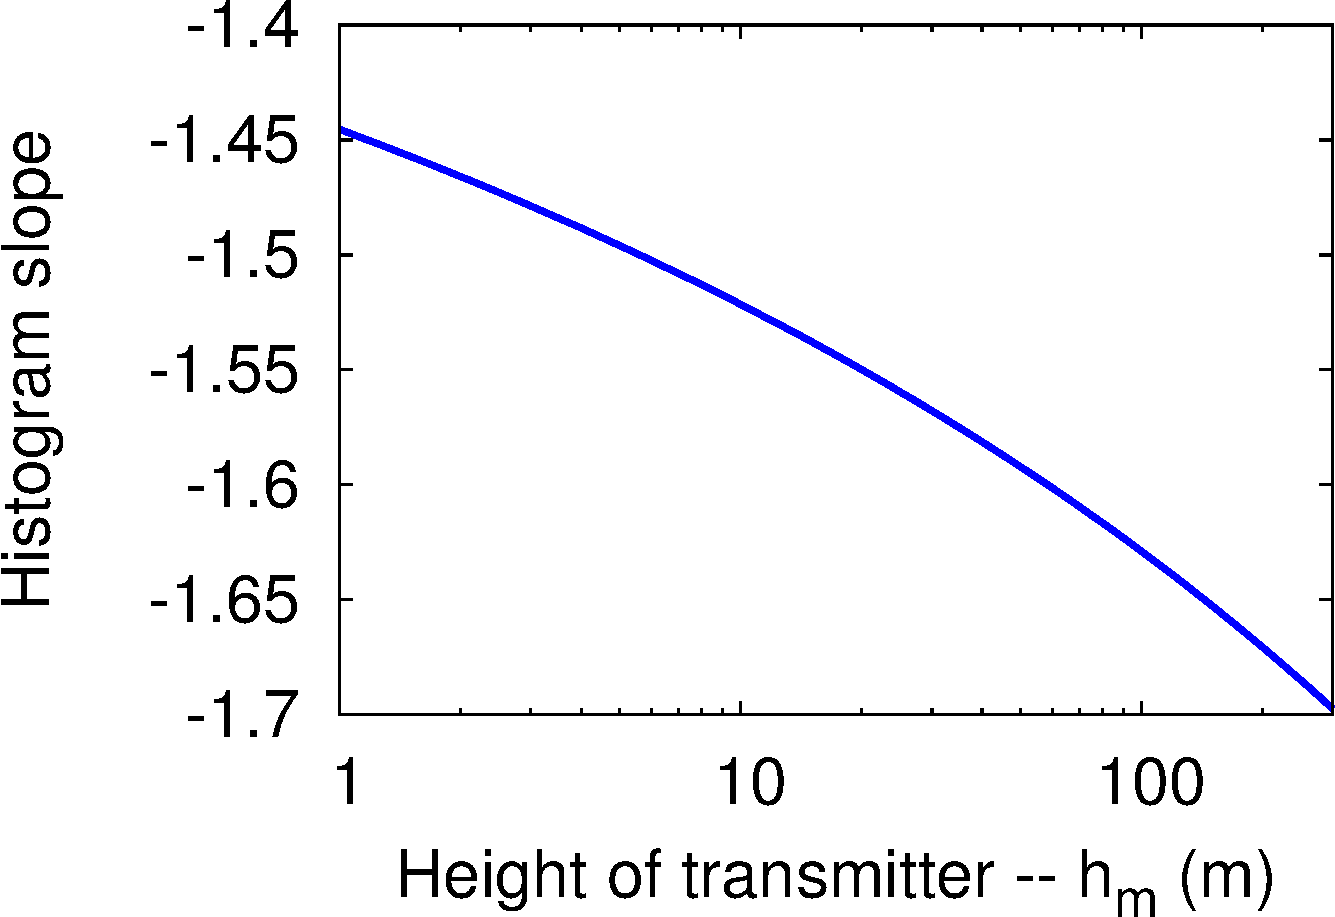
\includegraphics[width=6cm]{img/transmitter-height/plot-transmitter-height-trimmed}
\caption{Effect of transmitter height on the slope of a log-log histogram.}
\label{fig:plot-transmitter-height}
\end{center}
\end{figure}
This is valid for transmitters that have a height of 30--200 m, the range over which Hata's model was defined. This yields estimated distribution slopes of $-1.57$ and $-1.67$ for $30$ m and $200$ m high transmitters respectively. In Figure~\ref{fig:plot-transmitter-height}, the slope value is plotted as a function of the transmitter height, including extrapolated values for transmitter heights down to 1 m.

\subsection{Noise contribution} \label{sec:histogram-noise}
The full measured distribution will consist of the power-law distribution combined with that of the noise and the celestial signal. For now, we will ignore the contribution of the celestial signal, as its contribution to the amplitude distribution will be minimal when observing fields without strong sources. Noise, however, will have a contribution. The real and imaginary components of receiver noise are independent and identically Gaussian distributed. Consequently, an amplitude $x$ will be Rayleigh distributed: 
\begin{equation}\label{eq:rayleigh-formula}
f_\textrm{noise}(x) =
\begin{cases}
\frac{x}{\sigma^2} e^{\frac{-x^2}{2\sigma^2}} & x > 0, \\
0 & \textrm{otherwise.}
\end{cases}
\end{equation}
Because most of the samples will be unaffected by RFI, this will be the dominating distribution. The Rayleigh distribution is plotted together with the -2 power-law distribution of Eq.~\eqref{eq:two-dimensional-distribution} in Fig.~\ref{fig:rayleigh-and-rfi-distributions}.

\begin{figure}
\begin{center}\hspace{-5mm}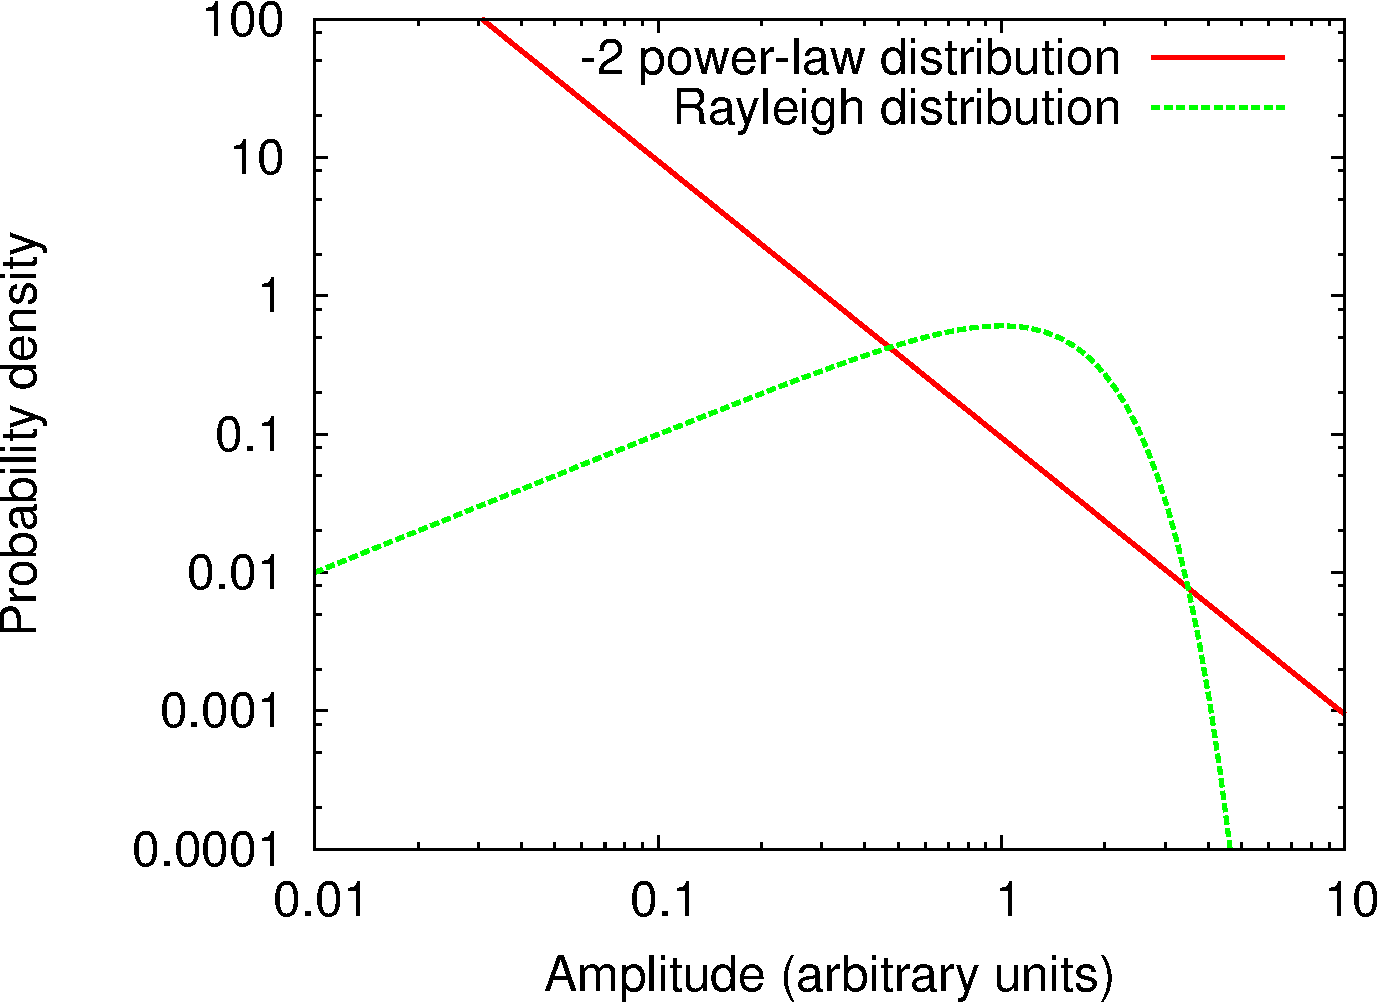
\includegraphics[width=8cm]{img/plot-rayleigh-and-rfi-trimmed}
\caption{The Rayleigh and power-law distributions in a log-log plot. The power-law distribution (Eq.~\eqref{eq:two-dimensional-distribution}) has a constant slope of -2. The slope of the Rayleigh distribution in the limit of the origin is 1. Its maximum occurs where the amplitude value equals its mode $\sigma$, which is 1 in this example. For higher amplitudes, its slope decreases exponentially.}
\label{fig:rayleigh-and-rfi-distributions}
\end{center}
\end{figure}

So far, these are the expected histograms for pure noise and pure RFI that propagates through free space. However, the measured distribution is a mixture of the two. A perfect RFI detector would separate the samples in two distributions; one that is not affected by RFI, and therefore contains noise only, and one that is the sum of RFI and noise. Real RFI detectors can separate these distributions to some extent, but due to false positives and false negatives, the histograms will get mixed nevertheless. Even more, we still need to take into account that the RFI classified samples are also affected by noise. Although this effect is moderate, because 'most' RFI samples are of much higher amplitude than what is added because of the noise, it is the low-level RFI samples which we are interested in, and the relative effect of noise on those samples is large.

\begin{figure}
\begin{center}\hspace{-2mm}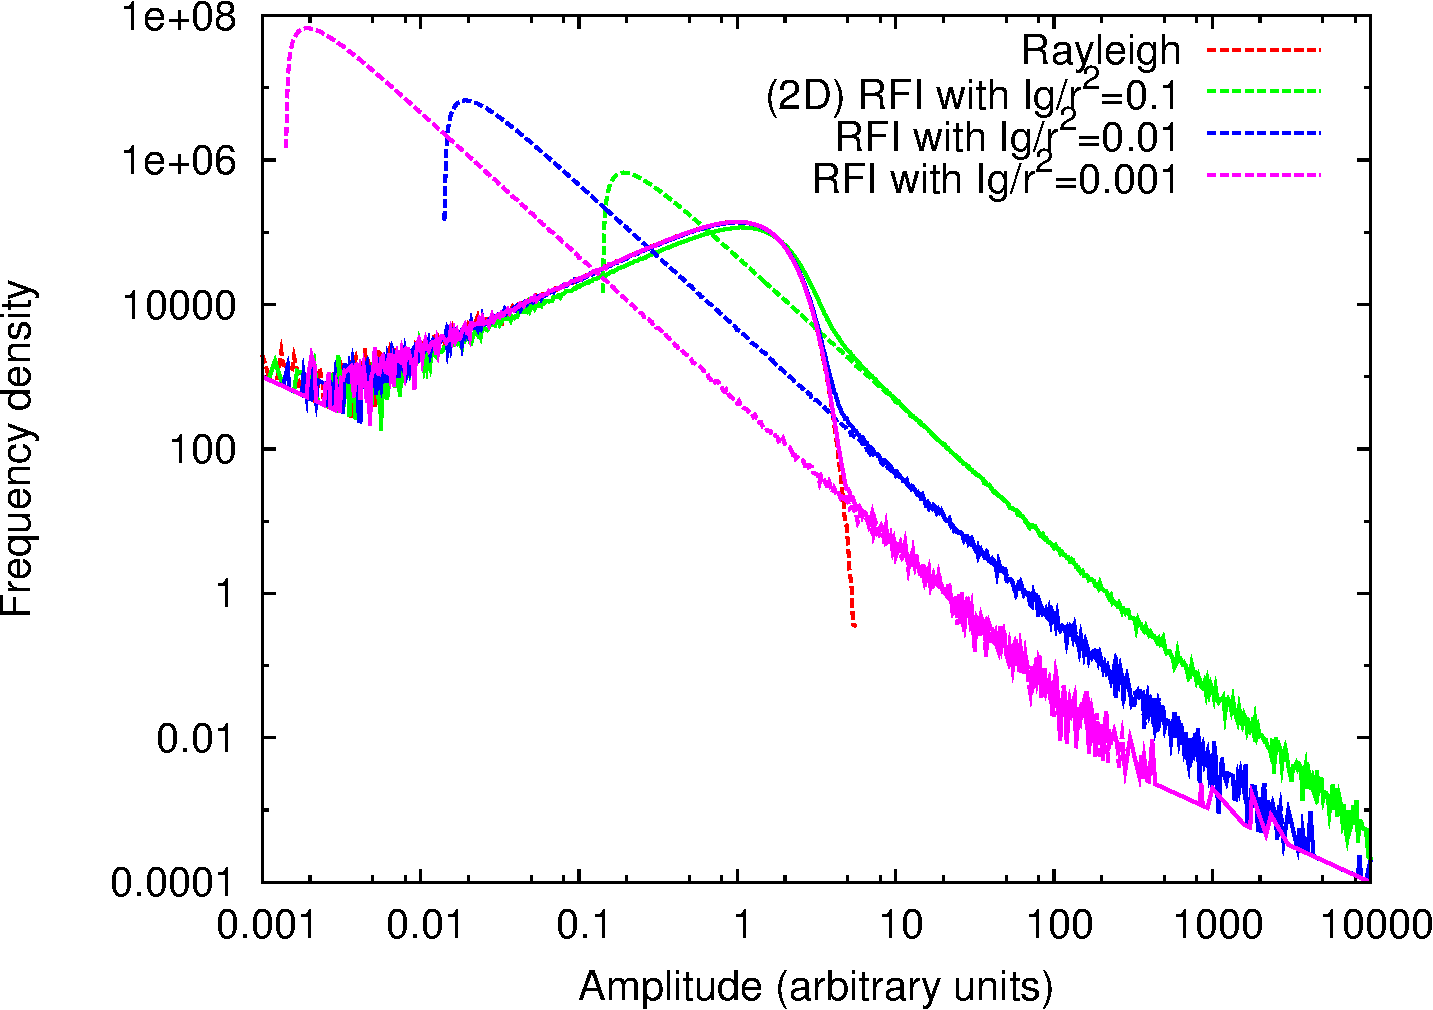
\includegraphics[width=8.5cm]{img/plot-rayleigh-and-rfi-combined-trimmed}
\caption{Histograms of simulated samples that all have a contribution of noise and RFI. Various settings of the parameters were used, and samples were drawn as described in Eq.~\eqref{eq:drawing-amplitudes}. Solid lines: the combined distributions, dashed lines: the original distributions before mixing. }
\label{fig:rayleigh-and-rfi-combined}
\end{center}
\end{figure}

To understand the distribution of samples consisting of RFI + noise, one needs to consider the individual contributions of the real and imaginary components. The real and imaginary components of samples that are affected by RFI, will follow a bivariate distribution: each complex component is the sum of a complex component of RFI and a noise sample. The noise comes from a Gaussian distribution with zero mean. The RFI distribution is assumed to be a power-law distribution with yet unknown exponent.

To calculate the corresponding amplitude distribution that is formed by the combination of the real and imaginary component distributions, it is easier to perform numerical simulations, as algebraic calculation is not trivial. The histogram can be numerically estimated by drawing complex real and imaginary samples from the two distributions and calculating and counting the amplitudes. A sample can be drawn from the RFI distribution by normalizing and inverting the cumulative frequency function in Eq.~\eqref{eq:cumulative-rfi-distribution} and evaluating it for a uniformly distributed variable. Note however that $F_{\textrm{amplitude}\le S}(S)$ is not limited; when decreasing the amplitude $S$ towards zero, the number of sources will go to infinity. Therefore, to draw a sample by using the inversion method, this would require a uniformly distributed variable $\sim U(0,\infty)$. By assuming that there are no samples beyond some limiting distance $r_L$, then $F_{\textrm{amplitude}\le S}(S) = N-c \pi r_L^2$ for $S < Ig/r_L^2$. Consequently, by sampling $x_u$ from a uniform distribution with $0 \le x_u \le N-c \pi r_L^2$ and applying the inverse of Eq.~\eqref{eq:cumulative-rfi-distribution}, we will sample amplitudes $S$ with $S \ge Ig/r_L^2$, and $S\sim$ the power-law distribution.

By normalizing $x_u$, a single complex RFI contaminated sample $S_{\textrm{RFI}}$ can be sampled with
\begin{equation} \label{eq:drawing-rfi-distribution}
\textrm{real}(S_{\textrm{RFI}})\leftarrow \frac{Ig}{x_u r_L^2}\textrm{,\hspace{1mm} imag}(S_{\textrm{RFI}}) \leftarrow \frac{Ig}{y_u r_L^2},
\end{equation}
with $x_u, y_u \sim U(0, 1)$, and the corresponding formula for drawing a sample $S$ that is contaminated by both RFI and noise is
\begin{equation} \label{eq:drawing-combined-distribution}
\textrm{real}(S) \leftarrow x_n + \frac{Ig}{x_u r_L^2}
\textrm{,\hspace{1mm} imag}(S) \leftarrow y_n + \frac{Ig}{y_u r_L^2},
\end{equation}
with $x_n \sim N(\mu=0; \sigma=1)$. Of course, the final amplitude sample $S_A$ can be calculated with 
\begin{equation} \label{eq:drawing-amplitudes}
S_A \leftarrow |S| = \sqrt{\textrm{real}({S})^2+\textrm{imag}({S})^2}.
\end{equation}
An example of distribution curves for various settings of $Ig/r_L^2$ is given in Fig.~\ref{fig:rayleigh-and-rfi-combined}.

If we assume that $I$, the average source strength; $g$, the average instrumental gain; and $r_L$, the distance over which those sources are visible, are all unknown, it can be seen from Eq.~\eqref{eq:drawing-combined-distribution} that given the histogram we can solve neither $r_L$, $I$ or $g$, as they all have the same effect of scaling the -2 power-law part of the histogram. Although calibration could in theory solve $g$, almost all sources will come in through the edges of the beam, and finding the expected values for the gains is therefore hard. The effects of these parameters on the histogram will be further discussed in \S\ref{sec:parameter-variability}.

Fig.~\ref{fig:rayleigh-and-rfi-combined} shows that the left side of the graph corresponds with the original Rayleigh distribution. From the right side of the histogram, we are able to estimate $Ig/r_L^2$, as the placing of the power-law curve is independent of the Rayleigh distribution for large $S$. Methods to constrain the parameters of the RFI distribution will be discussed in \S\ref{sec:rfi-distribution-constraints}. The curves in Fig.~\ref{fig:rayleigh-and-rfi-combined} are from histograms of samples that are all contaminated by both noise and RFI. In practice, we can not make this distinction accurately, as RFI detectors have a limited accuracy. Consequently, the observed histogram will be the sum of two types of histograms: the first histogram being contaminated by both noise and RFI, the second one only by noise.

% Exponential:
% fs(x):=c*%pi*I*g/x^2;
%
% Gaussian:
% fn(x):=1/(sqrt(2*%pi)*sigma)*exp(-x^2/(2*sigma^2));
%
% Convolution:
% fc(x):=romberg(fs(x)*fn(x+tau), tau, -inf, inf);
%
% plot2d([log(fc(x)),log(fs(x)),log(fn(x))], [x,0.01, 100], [y,-10,10], [logx]), sigma=1, I=1, g=1, c=1;

\subsection{Parameter variability} \label{sec:parameter-variability}
In reality, the parameters $c$, $I$ and $g$, which are the source density per unit area, source strength and instrumental gain respectively, will not be constant over time and frequency but have a stochastic nature. However, since each specific value for these parameters produces a power law, the combined distribution will still show a power law, as long as the parameters follow a distribution that is steep at high amplitudes (in $\log$--$\log$ space), such as a Gaussian or uniform distribution.

%\begin{figure}[tb]
%\begin{center}
%\includegraphics[width=12cm]{img/plot-passband.pdf}
%\caption{Effect of the low and high-band frequency responses on the amplitude histogram for different distributions.}
%\label{fig:plot-passband-histogram}
%\end{center}
%\end{figure}

One instrumental effect that is absorbed in $g$ is the frequency response of the instrument, i.e., the antenna response in combination with the passband of the analogue and digital filters. Because the data that are analysed in Sect.~\ref{sec:dist-results} have initially not been band-pass calibrated, the instrumental response is not uniform over frequency. We determined that the variation due to the band-pass is about one order of magnitude in the LBA and about a factor of two in the HBA.

The effect of the band-pass on the data distribution is consequently limited to one order of magnitude or less. If the RFI sources have an apparent power-law distribution with a certain exponent, the distribution will have a feature at low amplitudes due to the frequency response, but a power law with equal exponent will still appear when the distribution is observed over a wide enough range.

%In Fig.~\ref{fig:plot-passband-histogram}, the histograms of the frequency response are given. To also demonstrate the effect of mixing distributions, histograms are added for samples that are drawn from a uniform, Gaussian and -2 power-law distribution as in Eq.~\eqref{eq:drawing-rfi-distribution} with $Ig/r_L^2=1$, that have been multiplied by the passband. The frequency responses were determined by measuring the standard deviation of the data over frequency after flagging the data for interference. As expected, it can still be determined that the intrinsic distribution is a -2 power law.

Another effect that is absorbed in $g$, is the beam of the instrument. At the point of writing, LOFAR beam models are still being developed and are not yet well parametrized. However, since it is likely that most RFI sources are observed at the edges of the beam, it can be expected that the beam will have a limited effect on the histogram of an observation, comparable with the effect of the frequency response.

\section{Methods} \label{sec:distribution-methods}
In this section we will briefly discuss how the histograms are created, how the slope of the underlying RFI distribution is estimated and show how to constrain some of the intrinsic RFI parameters.

\subsection{Creating a histogram} \label{sec:histogram}
While creating a histogram is trivial, it is important to note that it is necessary to have a variable bin size. This is mandated by the large dynamic range of the histogram that we are interested in. Therefore, we chose to have a bin size that increases linearly with the amplitude $S$, and the frequency distribution is normalized by the bin size after counting. Consequently, in parts of the histogram that have a sparse number of samples, the outlying samples will follow a $1/S$ curve, or a -1 slope in a log-log plot. This can be seen in the tails of the distributions of Fig.~\ref{fig:rayleigh-and-rfi-combined}. This, however, is not an intrinsic feature of the data but a consequence of the binning method.

\subsection{Estimating $\sigma$ and slope parameters}
The mode $\hat\sigma$ of the Rayleigh distribution is estimated by finding the amplitude with the maximum occurrences, i.e., the amplitude corresponding to the peak of the histogram. The slope is estimated using linear regression over a visually selected interval.
%\begin{equation}
%R=\left[20\hat\sigma; 10^{\frac{1}{2}\left(\log_{10} 20\hat\sigma + \log_{10} S_\textrm{max}\right) } \right].
%\end{equation}
%In terms of the log-log histogram, the start of the interval corresponds with the point that is $1.3$ units to the right of the peak in the histogram, and the interval end corresponds with the point halfway between the start point and the maximum amplitude. This interval starts near the start of the RFI slope but past where the Rayleigh curve dominates. It also does not include the noisy data at the end of the curve. The curves are not always completely straight in this interval, but since we use the same stable way to determine the interval over which to calculate the slope, we can at least compare them.

One should note that fitting straight lines to the distribution curve in a log-log plot is not the most accurate way of estimating the exponent of a power-law distribution \citep{power-law-distribution}. However, because of our enormous sample size, which allows fitting the line over a large interval, the estimator will be sufficiently accurate for our purpose. Nevertheless, we will additionally calculate a maximum likelihood estimator for comparison. The maximum-likelihood estimator for the exponent in a power-law distribution is given by the Hill estimator \citep{hill-estimator, power-law-distribution}, defined as:
\begin{equation} \label{eq:hill}
 \alpha_H = 1 + N \left(\sum\limits_{i=1}^{N} \ln \frac{x_i}{x_\textrm{max}} \right)^{-1}.
\end{equation}
However, this estimator assumes the distribution is not cut-off at a high point. In our case, the distribution is cut-off at both sides, for example because of the limit of the analogue-digital converter (see \S\ref{sec:rfi-distribution-constraints}). Therefore, using this estimator will result in an estimate that is steeper (i.e., more negative) than the actual distribution. Moreover, the estimator requires an iteration over all data points, and because of the size of the data sets this is somewhat impractical. However, we can calculate Eq.~\eqref{eq:hill} by adding the bin centre values $N$ times to the calculation, where $N$ the bin frequency. Because our bin size is small and the distribution is well sampled, the resulting estimate will be close to the normal Hill estimator. This overcomes the need to iterate over all data.

\subsection{Determining RFI distribution limits} \label{sec:rfi-distribution-constraints}
In this section we will show methods to find $S_U$ and $S_L$, the upper and lower flux limits of the power-law distribution at which the power law breaks down. Once the exponent of the power-law part of the distribution is estimated with the previously discussed techniques, the distribution can be extrapolated to find a lower flux limit. Assume that we have found a power law with exponent $\alpha$ and factor $\beta$ over an amplitude region $[S_1 ; S_2]$, resulting in the following frequency density function $g$:
\begin{equation} \label{eq:amplitude-power-law}
g(S) = \beta S^\alpha.
\end{equation}
\begin{figure}
\begin{center}
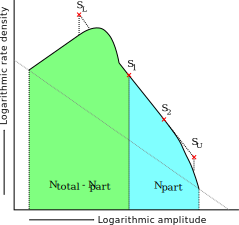
\includegraphics[width=7.5cm]{img/explanation-lower-constraint/FindingCounts}
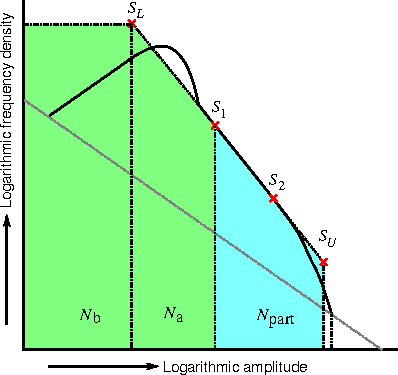
\includegraphics[width=7.5cm]{img/explanation-lower-constraint/FindingConstraints}
\caption{Cartoon of how a constraint on the lower fall-off point of the power-law distribution can be determined. Note that the labelled areas are areas as occupied in a linear plot, i.e., the integration of the density function. Areas in a log-log plot are not linearly related to the integral. There are two ways to estimate the lower constraint $S_L$: (i) the areas $N_a$ and $N_\textrm{total}-N_\textrm{part}$ are equal if $Ig/r^2$ is constant during the observation, and (ii) if one assumes $Ig/r^2\sim$ uniform, then $N_a+N_b = N_\textrm{total}-N_\textrm{part}$.}
\label{fig:explanation-constraints}
\end{center}
\end{figure}

Assume also that the histogram contains $N_\textrm{part}$ (RFI) samples with amplitude $> S_1$, as sketched in Fig.~\ref{fig:explanation-constraints}. The hypothetical upper limit $S_U$ of the distribution can now be found, i.e., the highest amplitude that would be observed when the distribution follows the power law up to that point, by solving
\begin{equation} \label{eq:upper-limit-constrained}
 \int\limits_{S_1}^{S_U} g(S) dS = N_\textrm{part}.
\end{equation}
In practice, the observed histogram will break down beyond some amplitude because of several reasons. First and most importantly, the samples themselves are digitized with an analogue-to-digital converter (ADC) with limited range. Second, we observe for a limited time and the frequency count is discrete. Because the chance of finding a sample with a very high intensity is low, it is unlikely to observe samples beyond some amplitude within the finite observing time. Finally, under the assumption of a uniform spatial distribution of RFI transmitters, samples with very high amplitude would have to be produced by transmitters that are very close to the telescope. However, it is likely that the uniform spatial distribution of transmitters will break down at closer distances.

Solving Eq.~\eqref{eq:upper-limit-constrained} results in
\begin{equation} \label{eq:upper-limit}
S_U = \sqrt[\alpha+1]{\frac{\alpha+1}{\beta} N_\textrm{part} + S_1^{\alpha+1}}.
\end{equation}
In some cases there will be no solution for $S_U$. This situation arises because the integral of the distribution function is finite even when $S_U \rightarrow \infty$. If $N_\textrm{part}$ exceeds the integrated value of the fitted distribution function, there is no solution. This can happen when the empirical distribution is not limited at the high end, or when it contains features that are not in the model.

Similar to the calculation of $S_U$ and by using $N_\textrm{total}$ as an upper limit to the total number of samples that are affected by the power-law distribution, one can estimate the lower limit $S_L$. For Fig.~\ref{fig:explanation-constraints} this means that the areas labelled $N_a$ and $N_\textrm{total}-N_\textrm{part}$ are equal. Solving this equality, one finds that
\begin{equation} \label{eq:lower-limit-1}
S_L = \sqrt[\alpha+1]{\frac{\alpha+1}{\beta}\left(N_\textrm{part} - N_\textrm{total} \right) + S_1^{\alpha+1}}.
\end{equation}

With the assumption that $Ig/r_L^2\sim$ a uniform distribution, the area labelled in Fig.~\ref{fig:explanation-constraints} as $N_b$ is also part of the RFI distribution, and a stronger constraint $\tilde S_L$ can be found by solving
\begin{equation}
 \int\limits_{\tilde S_L}^{S_U} g(S) dS + \tilde S_{L} g(\tilde S_{L}) = N_\textrm{total} - N_\textrm{part},
\end{equation}
which yields
\begin{equation} \label{eq:lower-limit-2}
\tilde S_L = \sqrt[\alpha+1]{ - \frac{1}{\alpha} \left( \frac{\alpha+1}{\beta} \left(N_\textrm{part} - N_\textrm{total}\right) + S_1^{\alpha+1} \right) }.
\end{equation}

With estimates of $\alpha$, $\beta$, $S_L$ and $S_U$, one has obtained a parametrization of the RFI distribution. As was shown in \S\ref{sec:histogram-noise}, the left-most point where the power-law distribution falls off is $Ig/r^2$ -- assuming free space propagation for the moment -- and therefore $S_L = Ig/r^2$. For Hata's propagation model, the more generic solution $S_L = \zeta Ig / r^\alpha$ is found. This value represents the apparent brightness of the sources that are the furthest away from the telescope. With a fully parametrized distribution of the effect of RFI sources, an empirical model for RFI effects can be made. Moreover, one can calculate $E(S_R)$, the expected apparent strength of RFI:
\begin{align} \label{eq:expected-value-rfi-def}
E(S_R) & = \frac{1}{N_{LU}}\int\limits_{S_L}^{S_U} \beta S^\alpha S dS
 = \frac{\beta}{N_{LU}} \left[ \frac{1}{\alpha+2} S^{\alpha+2} \right]_{S_L}^{S_U} \\
 & = \frac{\beta \left( S_U^{\alpha+2} - S_L^{\alpha+2} \right) }{N_{LU} \left( \alpha+2\right) }
\end{align}
Here, $N_{LU}$ is the number of samples between $S_L$ and $S_U$ after normalizing for the bin size:
\begin{align} \label{eq:n-between-sl-su}
N_{LU} = \int\limits_{S_L}^{S_U} \beta S^\alpha dS.
\end{align}
Substitution and simplification of these two results in
\begin{align} \label{eq:expected-value-rfi}
 E(S_R) & = \frac
{\left( S_U^{\alpha+2} - S_L^{\alpha+2}\right)\left(\alpha+1\right)} 
{\left(S_U^{\alpha+1} - S_L^{\alpha+1}\right) \left(\alpha+2 \right)}.
\end{align}
This is essentially the flux density that is caused by RFI without using RFI detection or excision algorithms. $E(S_R)$ has the same units as $S_L$ and $S_U$, thus after calibration (see \S\ref{sec:calibration}) could be given in Jy. In practice, the increase of system noise after correlation is much less severe because of RFI flagging, which excises a part of the RFI. One can assume that all RFI above a certain power level is found by the detector. Since modern RFI detection algorithms can find all RFI that is detectable ``by eye'' \citep{post-correlation-rfi-classification}, this power level will be near the level of the noise mode. In
\citet{lofar-radio-environment} % TODO correct citation if full citation available
the false-positives rate for the AOFlagger is estimated to be 0.5\%. An estimate of $S_d$, the average lower limit of detected RFI, can be calculated by finding the point on the distribution where the area under the distribution to the right of $S_d$ equals the real number (true positives) of RFI samples. Therefore, the limit is calculated similar to Eq.~\eqref{eq:lower-limit-1}, where the term $N_\textrm{part} - N_\textrm{total}$ needs to be replaced with $N_\textrm{RFI}$, which equals the total number of samples detected as RFI minus the 0.5\% false positives.

Finally, $E(S_\textrm{leak})$, which is the expected value of leaked RFI not detected by the flagger, can be calculated by replacing $S_U$ with $S_d$ in the numerator of Eq.~\eqref{eq:expected-value-rfi} and subtracting the removed number of samples from the total of number of samples. Assume that a fraction of $\eta$ samples are not detected as RFI and $1-\eta$ have been detected as RFI, then
\begin{align} \label{eq:expected-value-leaked-rfi}
E(S_\textrm{leak}) & = \frac{1}{\eta N_{LU}}\int\limits_{S_L}^{S_d} \beta S^\alpha S dS
= \frac{\left( S_d^{\alpha+2} - S_L^{\alpha+2} \right) \left( \alpha+1 \right) } {\eta \left( S_U^{\alpha+1} - S_L^{\alpha+1}\right) \left( \alpha+2 \right)}.
\end{align}
This is the average contribution that leaked RFI will have on a single sample. It has the same units as the parameters $S_L$, $S_U$ and $S_d$. Typical values for $\eta$ are $0.95$--$0.99$.

\subsection{Calibration} \label{sec:calibration}
We can assign flux densities to the horizontal axis of the histogram by using the system equivalent flux density (SEFD) of a single station. The current LOFAR SEFD is found to be approximately 3000~Jy for the HBA core stations and 1500~Jy for the remote stations in the frequency range from $125$--$175$ MHz. For all Dutch LBA stations, in the frequency range $40$--$70$ MHz the SEFD is approximately 30,000~Jy. The standard deviation $\sigma$ in the real and imaginary values is related to the SEFD with % TODO citation
\begin{equation}
 \sigma = \frac{\textrm{SEFD}}{\sqrt{2 \Delta \nu \Delta t}},
\end{equation}
where $\Delta \nu$ is the bandwidth and $\Delta t$ is the correlator integration time. The standard deviation will appear as the mode of the Rayleigh distribution. By fitting a Rayleigh function with fitting parameter $\sigma$ to the distribution, one finds the corresponding flux density scale.

RFI sources will enter through the distant sidelobes of the station beams from many unknown directions. Moreover, models for the full beam are often hard to construct. Therefore, we will not try to calibrate the beam, and the flux densities in the histogram are apparent quantities. Consequently, we will not be able to say something about the true intrinsic power levels of RFI sources.

\subsection{Error analysis}
An estimate for the standard deviation of the slope estimator $\hat \alpha$ can be found by calculating $\textrm{SE}(\hat \alpha)$, the \emph{standard error} of $\hat \alpha$. The standard error of the slope of a straight line \citep[pp. 32--35]{acton-analaysis-of-straight-lines} is given by
\begin{equation} \label{eq:stderr-slope}
 \textrm{SE}(\hat \alpha) = \sqrt{\frac{SS_{yy}-\hat\alpha SS_{xy}}{\left(n - 2\right) SS_{xx}}},
\end{equation}
where $SS_{xx}$, $SS_{xy}$ and $SS_{yy}$ are the sums of squares, e.g., $SS_{xy}=\sum_{i=1}^n (x_i - \bar x) (y_i - \bar y)$ and $n$ is the number of samples. However, we found that this is not a representative error in our case, because the errors in the slope are not normally distributed. The noise in the part of the histogram over which the slope is calculated, is very small due to the large amount of samples. Consequently, the estimated standard deviation of $\hat \alpha$ is very low. Nevertheless, when the slope is calculated over subsections of the original range over which the slope is calculated, one finds the line is not completely straight and the slope is changing more than is predicted by the standard error. Therefore, we introduce an error estimate $\epsilon_\alpha$ that quantifies a normalized standard deviation of the slope over the range. This error is formed by calculating the slope over $n_\alpha$ smaller subranges in the histogram, creating $n_\alpha$ estimates $\alpha_i$. If the errors in $\alpha_i$ are normally distributed with mean zero, the standard deviation over the full range will be $\sqrt{n_\alpha}$ times smaller. Therefore, an estimate of the variance of $\hat \alpha$ can be calculated with
\begin{equation}
 \epsilon_{\hat\alpha} = \sqrt{\frac{\sum \left( \alpha_i - \hat\alpha \right)^2 }{n^2_\alpha - n_\alpha}}.
\end{equation}
This estimate is slightly depending on the number of subranges that is used, $n_\alpha$, because the errors are not Gaussian distributed, but we found that $\epsilon_{\hat\alpha}$ is more representative than the standard error of $\hat\alpha$. 

The Hill estimator of Eq.~\eqref{eq:hill} is a different estimation method for the exponent in the power-law distribution, and yields therefore also a different standard error. The standard error of the Hill estimator is \citep{power-law-distribution}
\begin{equation} \label{eq:stderr-hill}
 \textrm{SE}(\hat \alpha_H) = \frac{-\alpha - 1}{\sqrt{n}} + \mathcal{O}(\frac{1}{n}).
\end{equation}
Because the number of samples is very large ($>10^{11}$), the $\mathcal{O}$-term will be very small. Therefore, we will calculate the quantity without this term. As with the standard error for the slope of a straight line in Eq.~\eqref{eq:stderr-slope}, the standard error for the Hill estimator yields very small quantities. Again, this is because it assumes the underlying power law has a fixed exponential, while in our case the power law seems to vary. Therefore, this value is given only for completeness.

Because our distributions are huge, we decided not to do goodness-of-fit tests, because these require many similar distributions to be simulated in order to reach accurate decision. Instead, we will try to evaluate the distributions visually.

\section{Data description} \label{sec:dist-data}
We have analysed the distributions of two data sets. Both data sets are 24 h LOFAR RFI surveys and are extensively analysed in
\citet{lofar-radio-environment}. % TODO
In one set, the low-band antennae (LBA) were used and the frequency range 30.1--77.5 MHz was recorded, while in the other the high-band antennae (HBA) were used to record the frequency range 115.0--163.3 MHz. More stations were used in the LBA set. The specifications of the two sets are listed in Table~\ref{table:dist-data-specs}. The stations that have been used are geometrically spread over an area of about 80~km and 30~km in diameter at maximum for the LBA and HBA sets respectively.

Although we have used Hata's model to estimate the RFI log-log histogram slope, our frequency range falls partly outside the frequency range over which Hata's model has been verified. However, according to Hata's model the observing frequency does not influence the power-law exponent in the frequency range 150--1500 MHz, thus it can be assumed the exponent will at least not significantly differ over the HBA range.

To detect RFI, the AOFlagger \citep{post-correlation-rfi-classification, LOFAR-RFI-pipeline, scale-invariant-rank-operator} was used. However, since this flagger is partly amplitude-based, it is likely that low-level RFI will leak through the detector. Since it is also low-level RFI we are interested in, we will analyse unflagged data and the RFI classified data.

\begin{table}
\caption{Data set specifications}\label{table:dist-data-specs}
\begin{center}
\begin{tabular}{lrr}
                    & \textbf{LBA set}& \textbf{HBA set} \\
\hline
\hline
Observation date    & 2011-10-09      & 2010-12-27 \\
Start time          & 06:50 UTC       & 0:00 UTC \\
Length              & 24 h           & 24 h \\
Time resolution     & 1 s             & 1 s \\
\hline
Frequency range     &  30.1--77.5 MHz & 115.0--163.3 MHz\\
Frequency resolution & 0.76 kHz    & 0.76 kHz \\
Number of stations  &  33           & 13 \\
Total size          & 96.3 TiB        & 18.6 TiB \\
\hline
Field               & NCP             & NCP \\
Amount RFI detected & 1.77\%       & 3.18\% \\
\hline
\hline
\end{tabular}
\end{center}
\end{table}

\begin{figure*}
\begin{center}
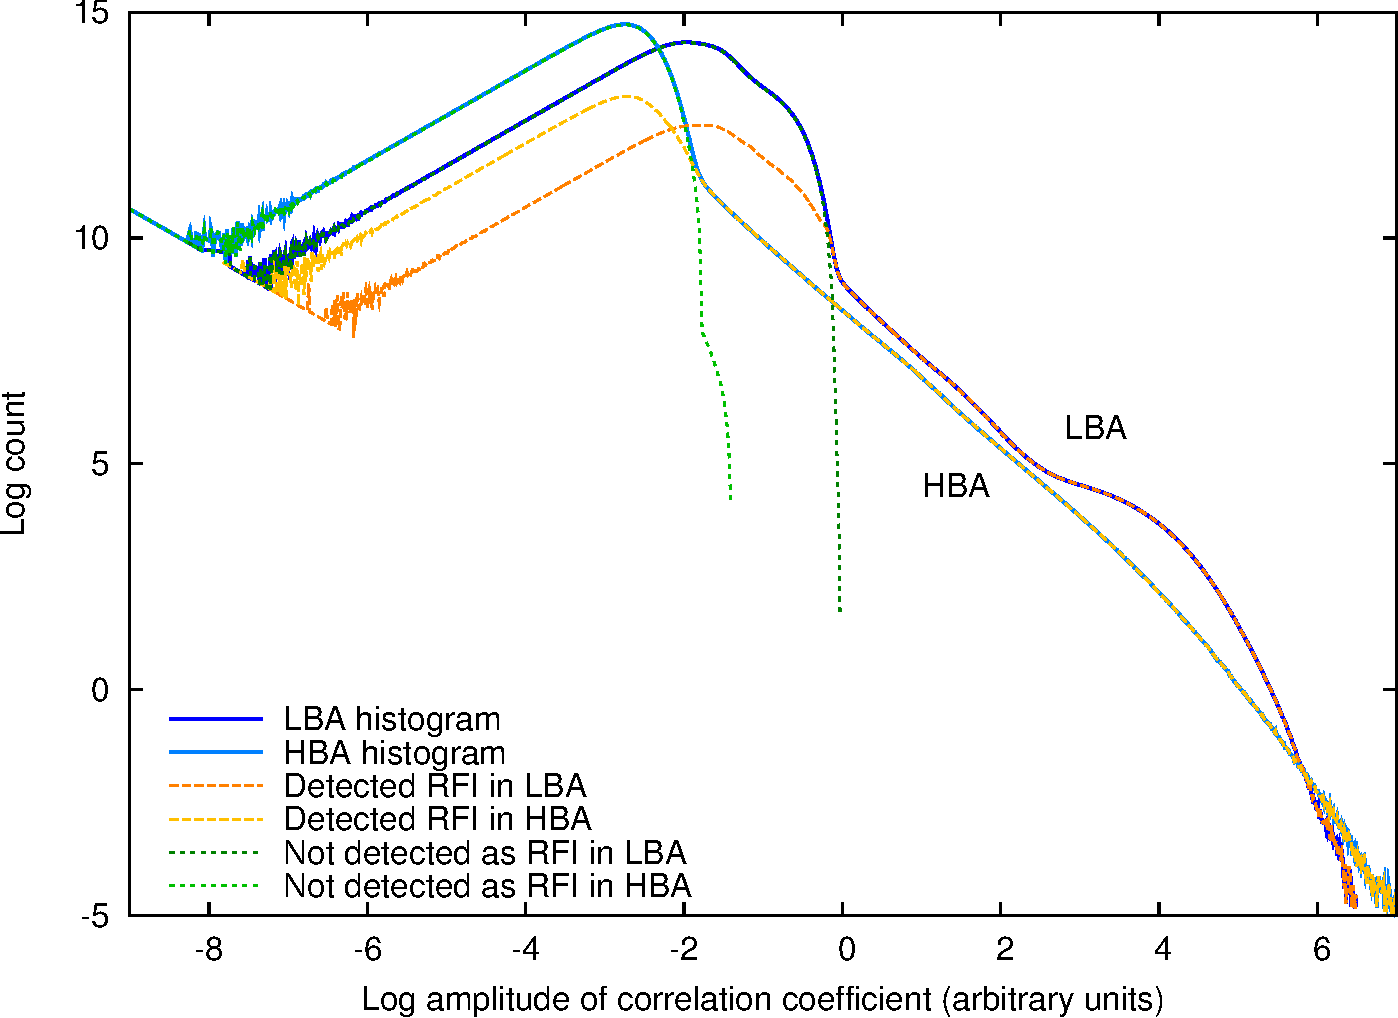
\includegraphics[width=12cm]{img/histograms-raw-trimmed}
\caption{The histograms of the two data sets before pass-band correction and flux calibration.}
\label{fig:Histograms-raw}
\end{center}
\end{figure*}

\section{Results} \label{sec:dist-results}
In this section we present the histograms of the LBA and HBA sets and the results that were obtained by applying the methodology discussed in Sect.~\ref{sec:distribution-methods}. 

\begin{figure}
\begin{center}
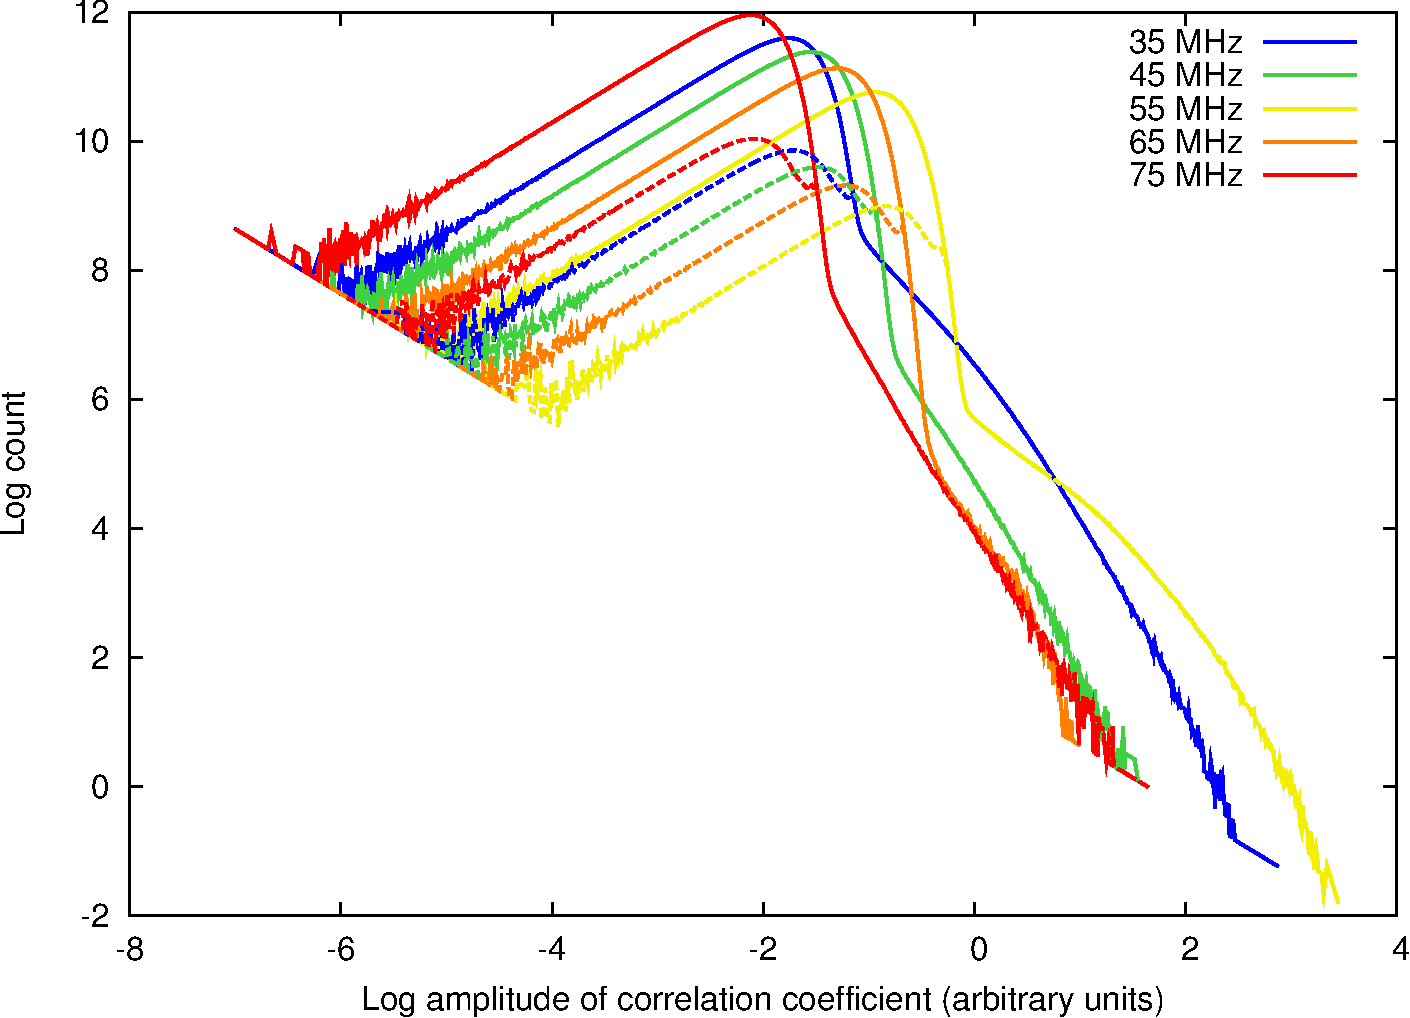
\includegraphics[width=8cm]{img/plot-lba-dist-per-frequency-trimmed}
\caption{Histograms for $5$ different $0.2$ MHz LBA sub-bands without pass-band correction and flux calibration. The continuous lines represent the data before RFI flagging. The dashes lines are the histograms of the samples that have been classified as RFI.}
\label{fig:plot-dist-per-frequency-LBA}
\end{center}
\end{figure}

\subsection{Histogram analysis}
Fig.~\ref{fig:Histograms-raw} shows the histograms with logarithmic axes for the LBA and HBA sets. In both sets, it is clear that at least one variate with a Rayleigh and one with a power-law distribution have been observed. The left part of the histogram matches the Rayleigh distribution well up to the mode of the distribution. The bulge around the mode of the LBA histogram is wider due to the larger effect of the antenna response as discussed in \S\ref{sec:parameter-variability}. As can be seen in Fig.~\ref{fig:plot-dist-per-frequency-LBA}, the Rayleigh-bulges of individual sub-bands are not that wide, but they are not aligned because of the differing noise levels. This effect is not so strong in histograms of the HBA sub-bands in Fig.~\ref{fig:plot-dist-per-frequency-HBA}, because the HBA antenna response changes less over frequency.

\begin{figure}
\begin{center}
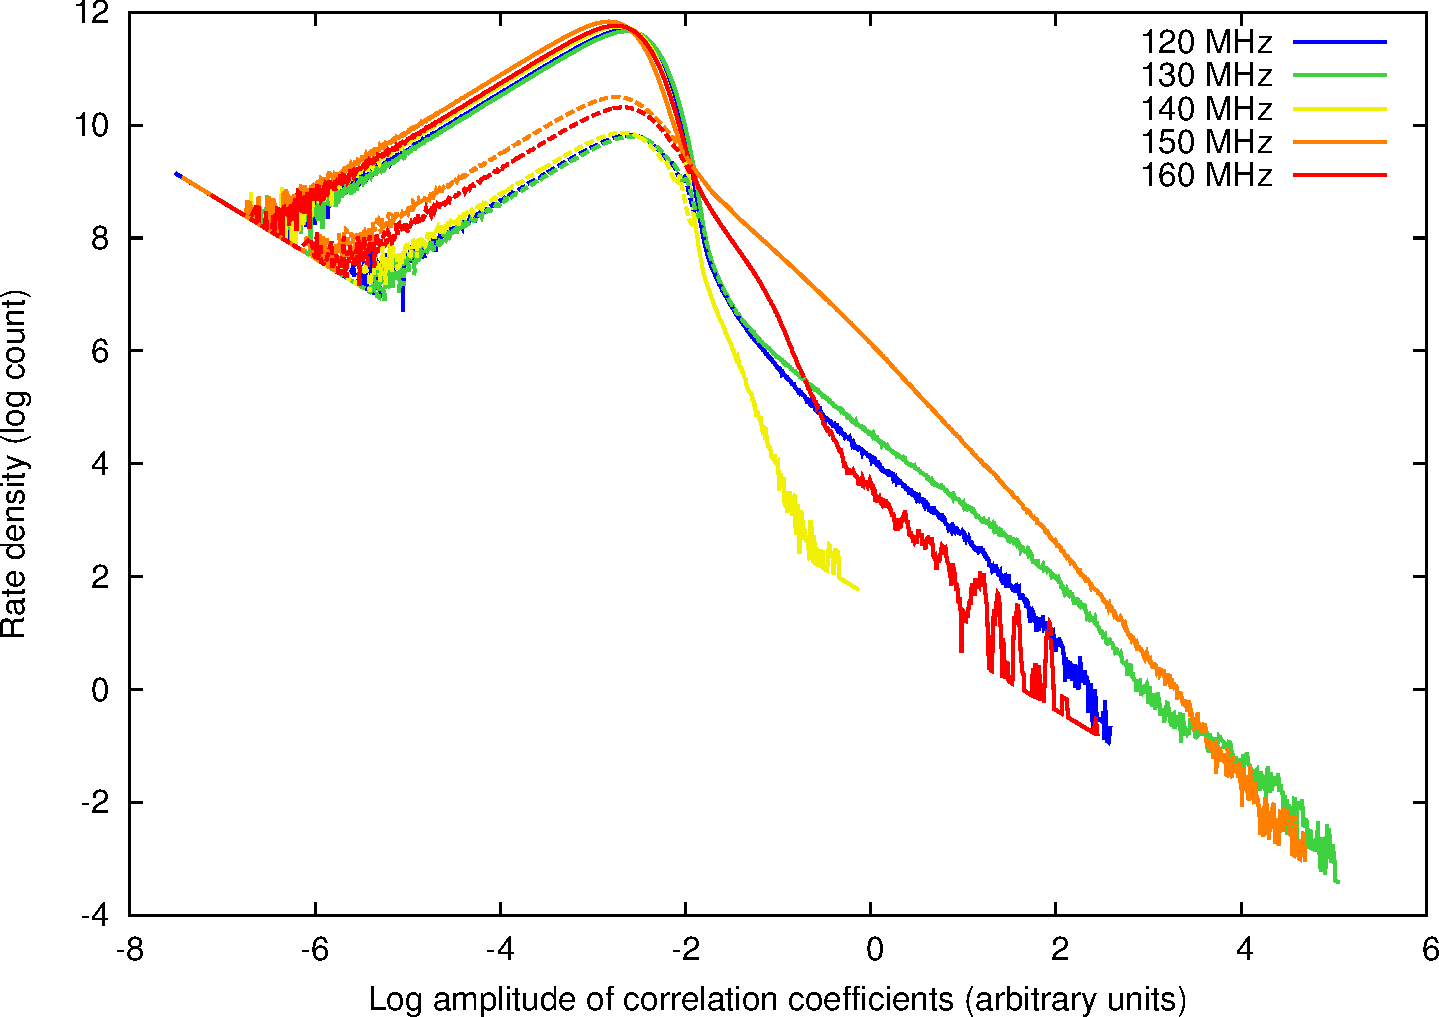
\includegraphics[width=8cm]{img/plot-hba-dist-per-frequency-trimmed}
\caption{Histograms for $5$ different $0.2$ MHz HBA sub-bands without pass-band correction and flux calibration. The continuous lines represent the data before RFI flagging. The dashes lines are the histograms of the samples that have been classified as RFI.}
\label{fig:plot-dist-per-frequency-HBA}
\end{center}
\end{figure}

It is to be expected that the RFI-dominated part of the distributions at different frequencies will reflect the underlying source populations. Both Figs.~\ref{fig:plot-dist-per-frequency-LBA} and \ref{fig:plot-dist-per-frequency-HBA} show that the power-law part of the distributions are very different for different sub-bands. Nevertheless, combining the data of all the sub-bands results in reasonably-stable power-law distributions. This indicates that the individual sub-bands have an approximately similar underlying power-law distribution, that is not yet apparent because not enough samples are combined in the histograms of individual sub-bands.

\begin{figure*}
\begin{center}
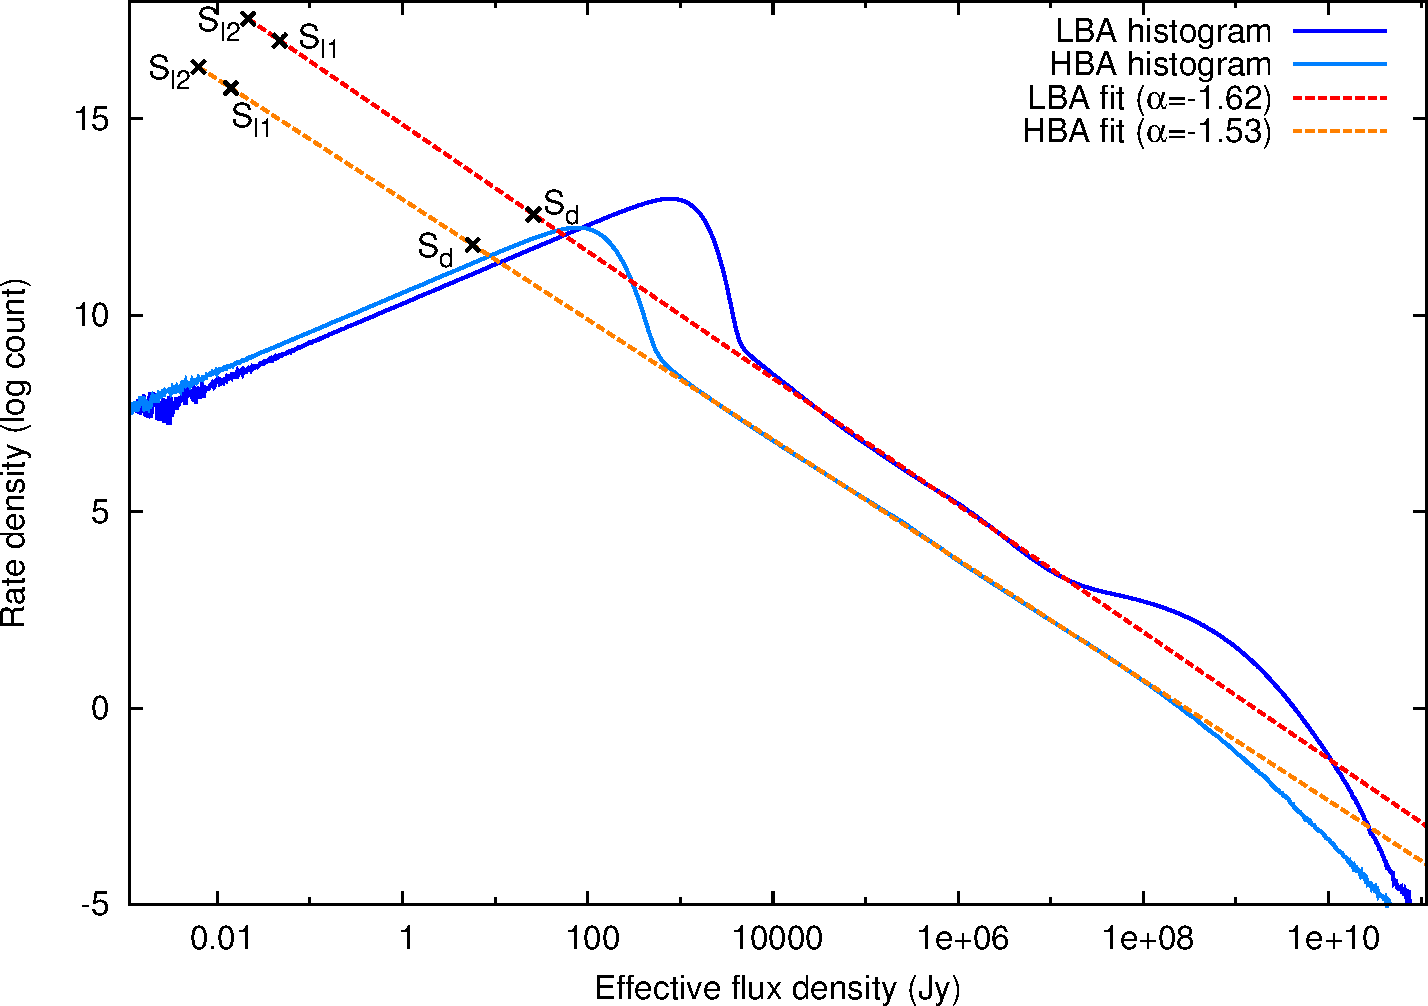
\includegraphics[width=13cm]{img/histograms-corrected-trimmed}
\caption{Observed LBA distribution after pass-band correction and flux calibration. $S_{l1}$ and $S_{l2}$ denote the limits of the distribution with a sharp lower cut-off (Eq.~\eqref{eq:lower-limit-1}) and uniform lower limit (Eq.~\eqref{eq:lower-limit-2}), $S_d$ is the average lower limit of RFI that is detected.}
\label{fig:histogram-passband-corrected}
\end{center}
\end{figure*}

To make sure that the antenna response does not influence the result of the slope, we have also analysed the curves after a simple band-pass calibration. This was performed by dividing each sub-band by its standard deviation after RFI excision. Because the standard deviation of the distribution might be affected by the RFI tail of the distribution, we compare the two histograms to make sure the power-law distribution is not significantly changed. The resulting histograms are shown in Fig.~\ref{fig:histogram-passband-corrected}. This procedure makes the bulge of the LBA histogram similar to the bulge of a Rayleigh curve and extends the power-law part. Nevertheless, it does not change the log-log slope of the power law in either histograms. This validates that the variable gain that is caused by the antenna response does not change the observed power law. Consequently, it can be expected that other stochastic effects, such as the intrinsic source strength and the beam gain due to a differing direction of arrival, will similarly not effect the power law. Because the pass-band corrected histograms provide a more representative analysis, we will use the corrected histograms for further analysis.

\begin{figure*}
\begin{center}
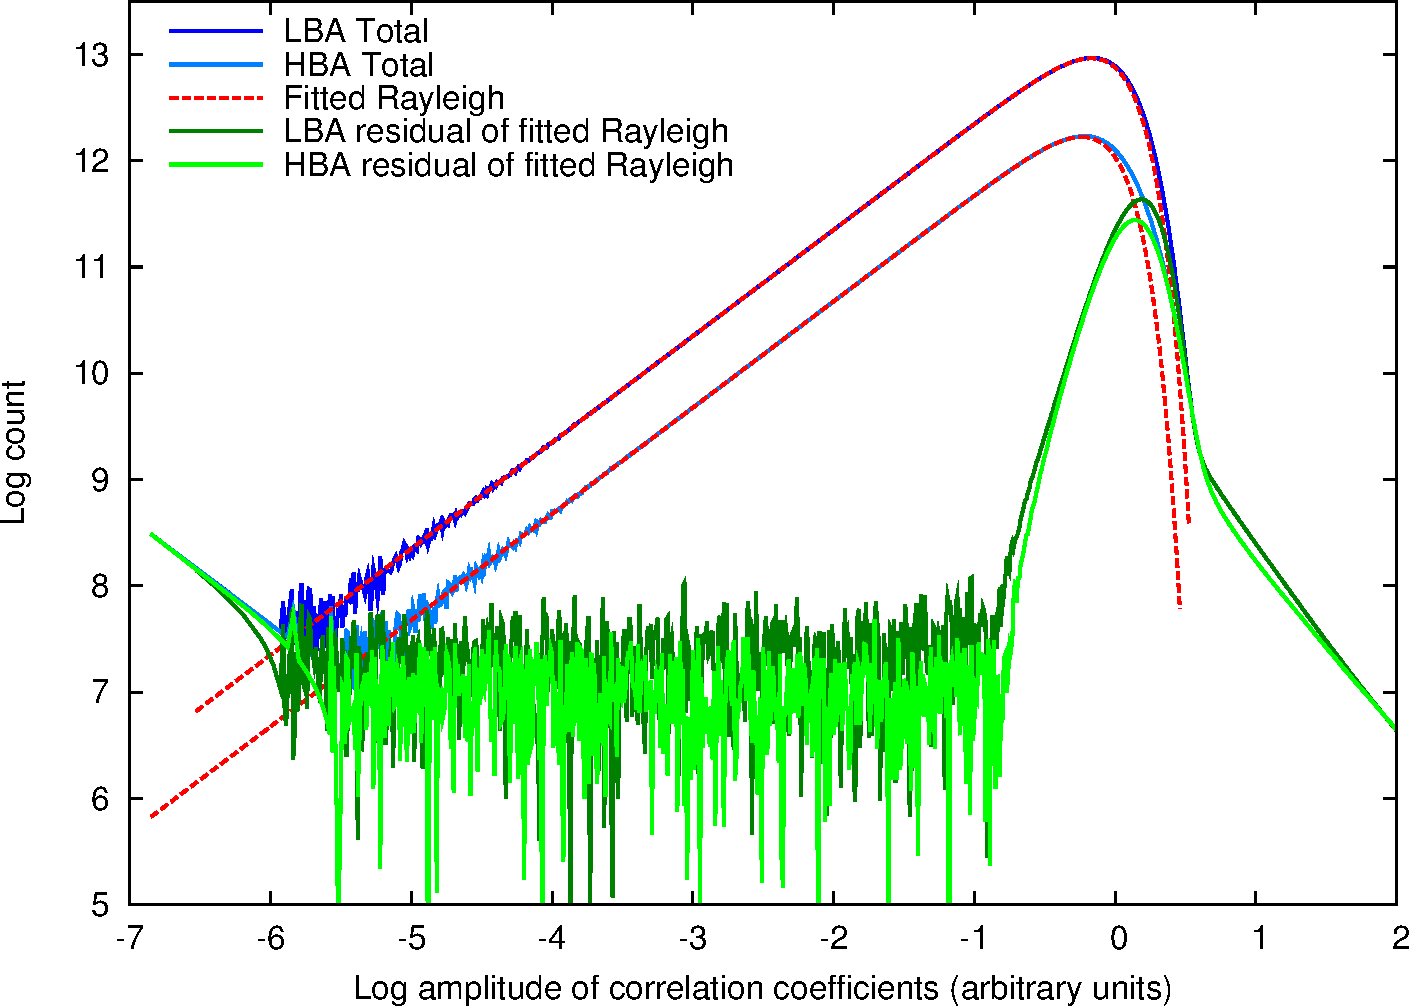
\includegraphics[width=13cm]{img/histograms-with-fits-trimmed}
\caption{Least-squares fits of Rayleigh distributions to the observed LBA and HBA histograms, after pass-band correction but without flux calibration.}
\label{fig:histograms-with-fits}
\end{center}
\end{figure*}

The Rayleigh parts of the distributions are plotted in Fig.~\ref{fig:histograms-with-fits}, along with a least-squares fit and its residuals. Both histograms follow the Rayleigh distribution for about five orders of magnitude, which is validated by the residuals that show only noise. It breaks down about one order of magnitude before the mode of the distributions. This is because of the multi-variate nature of the distributions, as was described in \S\ref{sec:histogram-noise}.

\begin{figure*}
\begin{center}
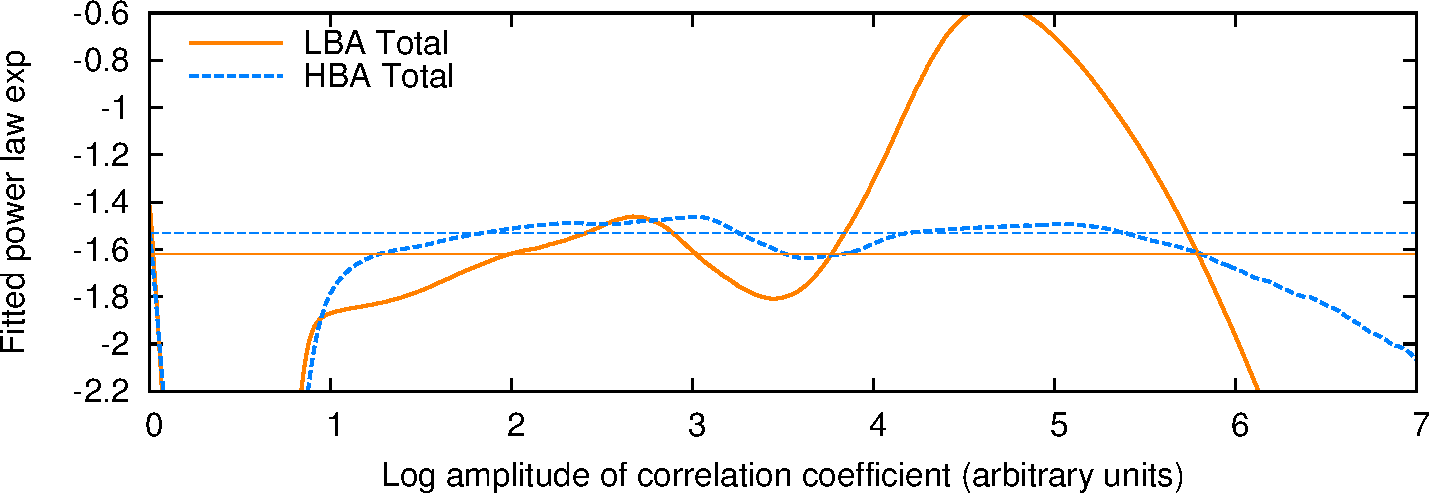
\includegraphics[width=13cm]{img/slopes-trimmed}
\caption{The slope of the band-pass corrected log-log histogram as a function of the brightness. The horizontal lines indicate the fitted slope over the full (semi-) stable region. The horizontal axis is not calibrated.}
\label{fig:plot-slopes}
\end{center}
\end{figure*}

If we go back to Fig.~\ref{fig:histogram-passband-corrected}, we see that in the LBA the power law is stable for about three orders of magnitude, and one order more in the HBA. Fig.~\ref{fig:plot-slopes} shows the slope of the log-log plot as a function of amplitude, which was constructed by performing linear regression in a sliding window, with a window size of 1 decade. The HBA shows very little structure in the slope, but the LBA is less stable and shows some features in its power-law part. Linear regression on the power-law part of the log-log plot results in a slope of $-1.62$ for the LBA and $-1.53$ for the HBA. These and the other derived quantities have been summarized in Table~\ref{table:dist-data-quantities}. Although the HBA slope does not show any other significant features besides the Rayleigh and power-law curves, the LBA power law ends with a bulge around an amplitude of $10^6$. This bulge is caused by a very strong source affecting lots of samples, and is a single outlier in the spatial distribution. We found this is caused by RFI observed for about an hour in the late afternoon in the lower LBA frequency regime, around $30$--$40$~MHz. Leaving this frequency range out flattens the bulge significantly, but does not completely eliminate it, because the source turned the receivers in non-linear state, causing leakage at lower intensity levels in the other sub-bands. Unlike linear regression, the fitting region of the Hill estimator is not limited at the high end. Consequently, because of the bulge, the Hill estimator evaluates for the LBA into a slope that is less steep, with a value of $-1.53$. For the HBA set, the Hill estimator is equal to the $-1.53$ value found by linear regression.

%\begin{figure}[tbp]
%\begin{center}
%\includegraphics[width=12cm]{img/plot-slope-over-frequency-trimmed}
%\caption{Slope of the log-log histogram slope over frequency in the LBA set.}
%\label{fig:plot-slope-over-frequency-LBA}
%\end{center}
%\end{figure}

%\begin{figure}[tbp]
%\begin{center}
%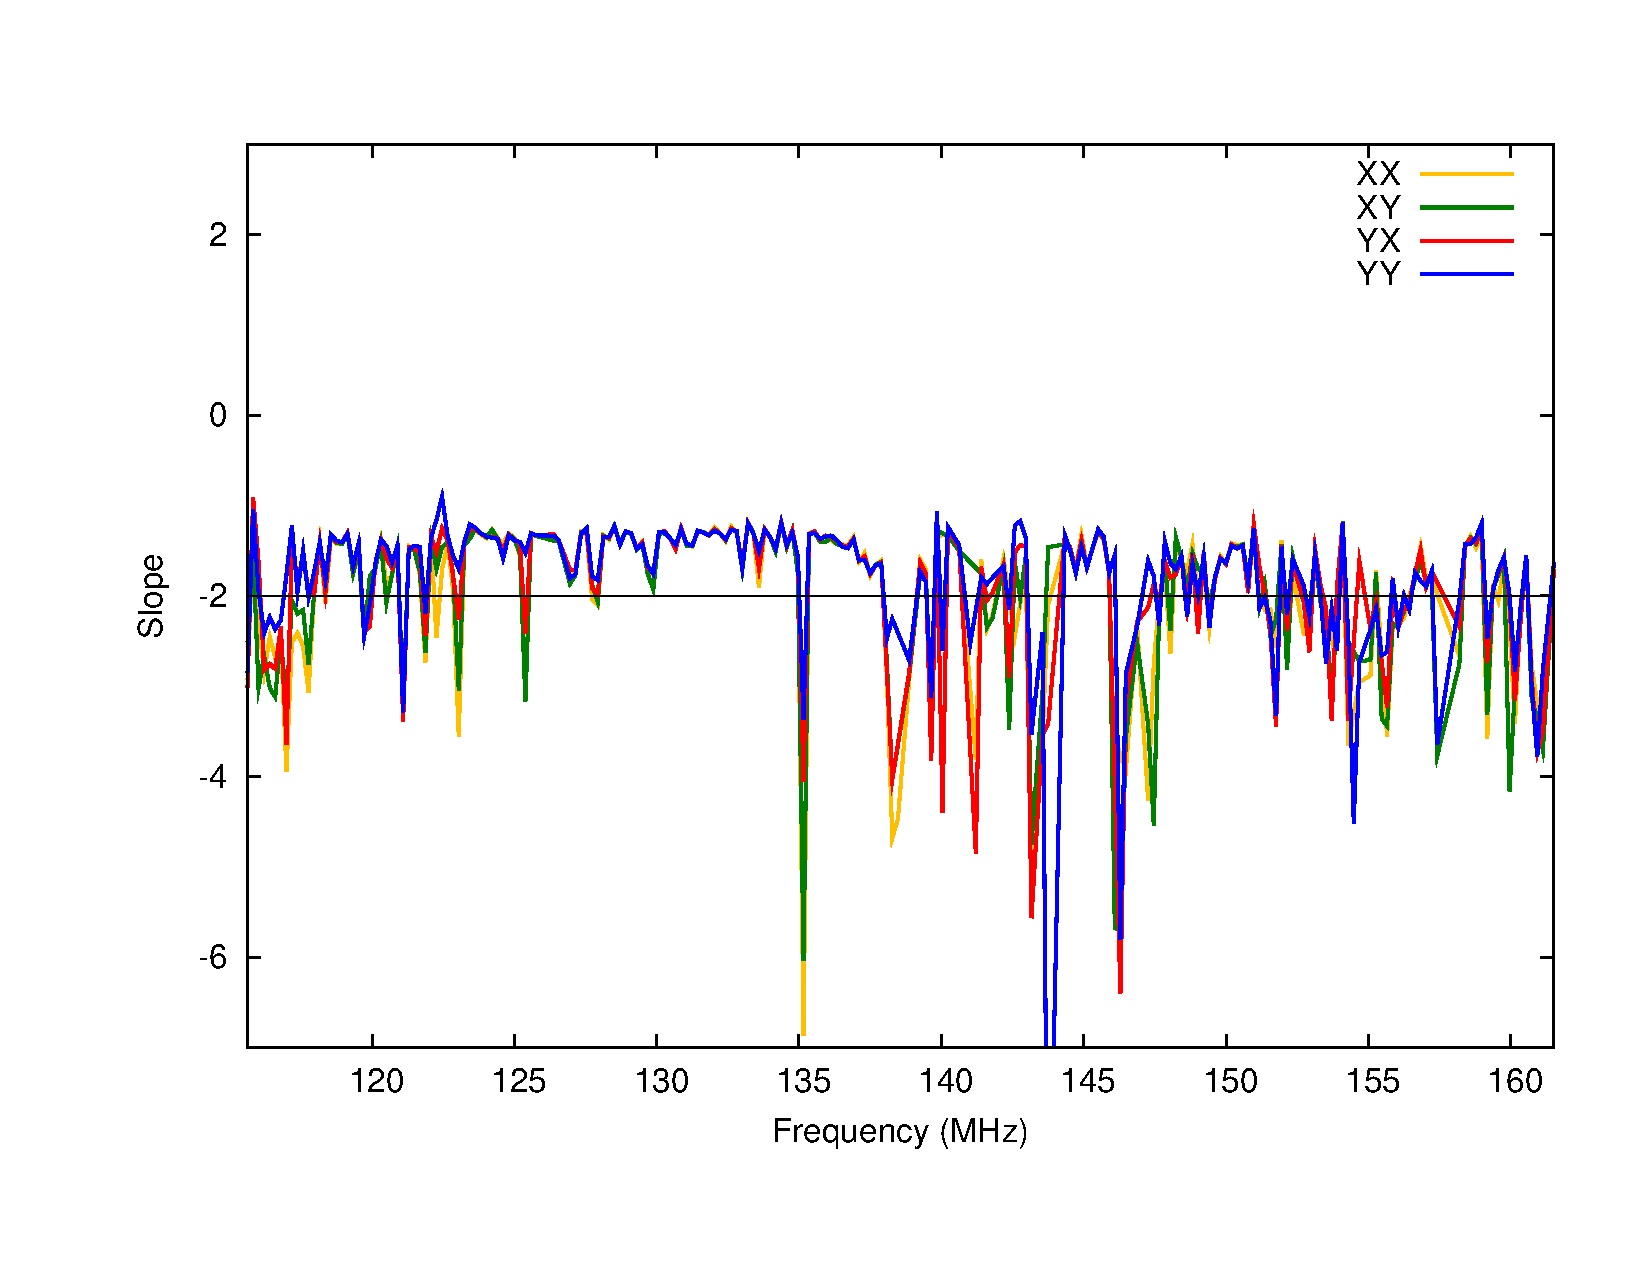
\includegraphics[width=12cm]{img/slope-over-frequency-HBA/plot-slope-over-frequency}
%\caption{Slope of the log-log histogram over frequency in the HBA set.}
%\label{fig:plot-slope-over-frequency-HBA}
%\end{center}
%\end{figure}

%\begin{figure}[tbp]
%\begin{center}
%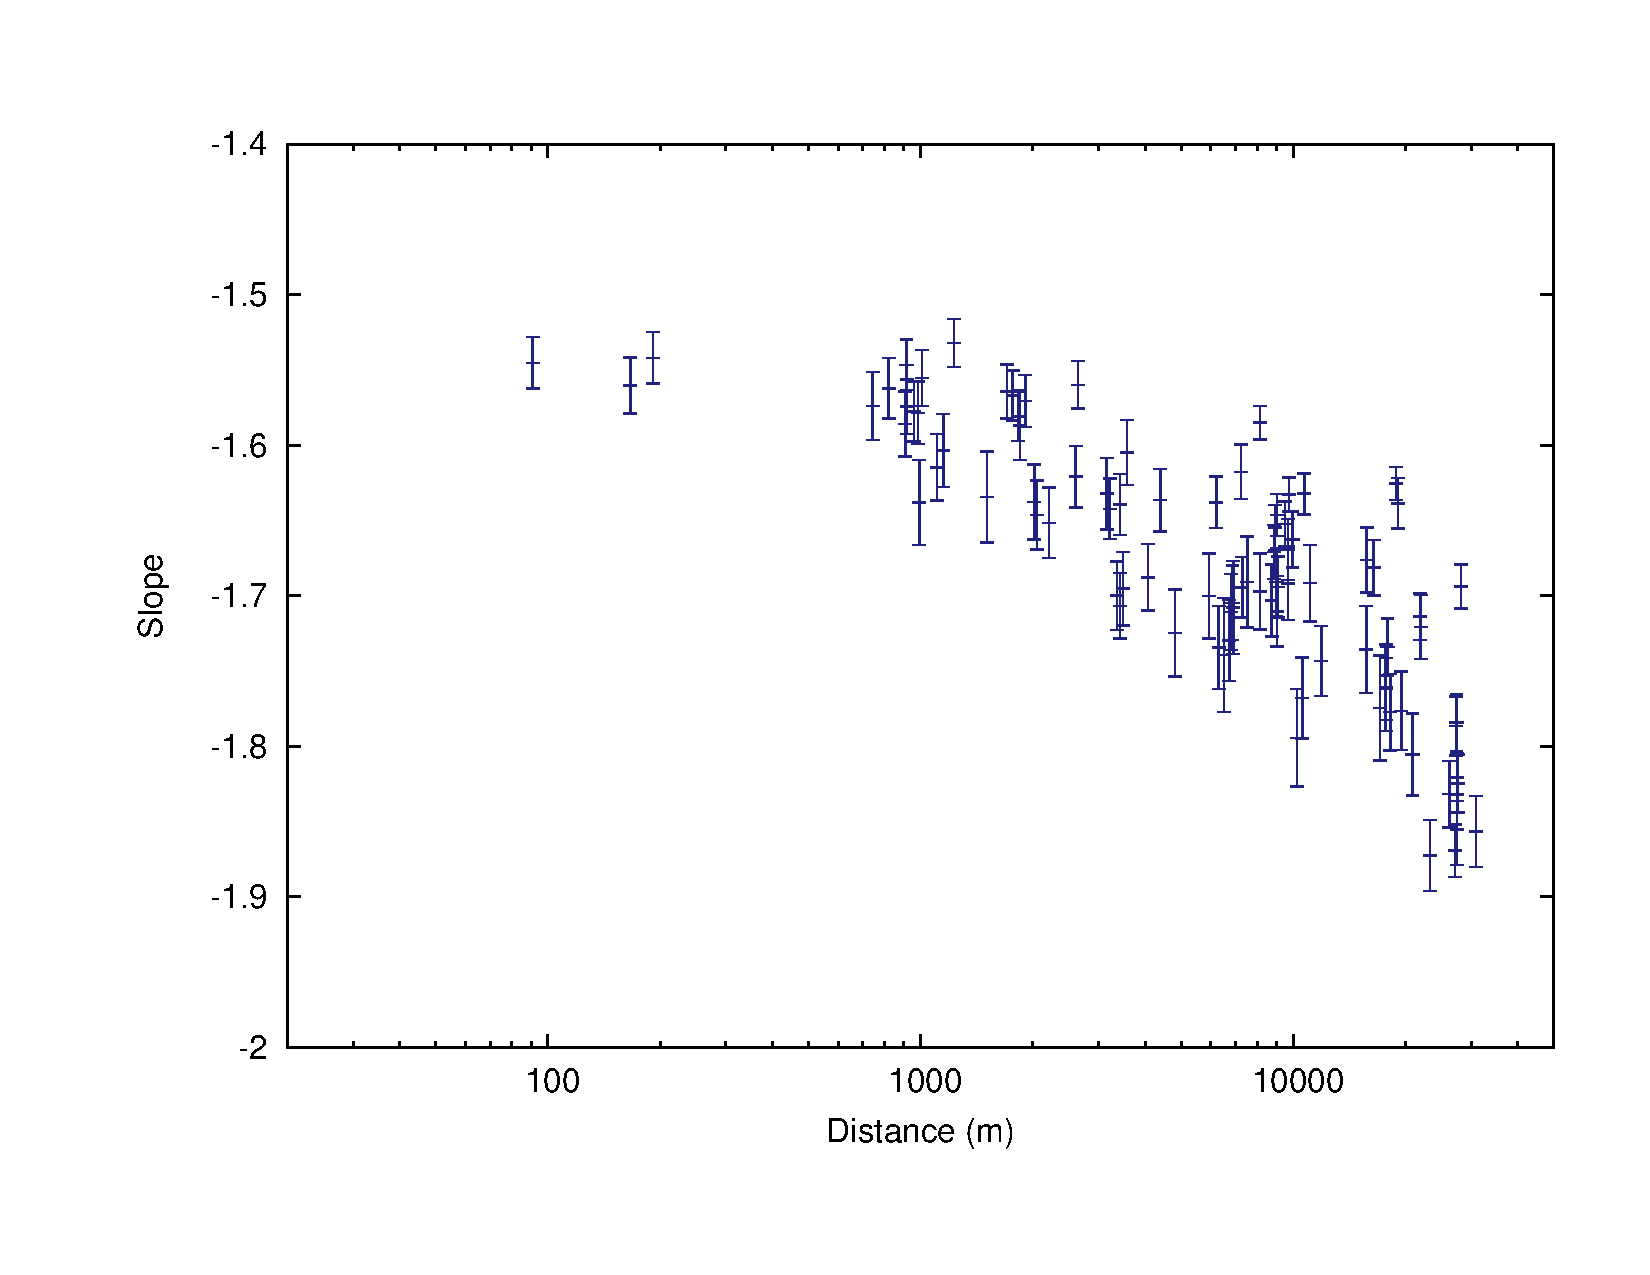
\includegraphics[width=12cm]{img/slope-over-baseline-HBA/plot-slope-over-baseline-wstddev}
%\caption{Slope of the log-log histogram over the baseline length for the HBA set. A single sub-band at 150 MHz was used. Error bars indicate $5\sigma$ level.}
%\label{fig:plot-slope-over-baseline-HBA}
%\end{center}
%\end{figure}

\begin{table*}
\centering
\begin{minipage}{12cm}
\caption{Estimated distribution quantities per data set. }\label{table:dist-data-quantities}
\begin{tabular}{@{}llrr@{}}
\textbf{Symbol} & \textbf{Name} & \textbf{LBA set}& \textbf{HBA set} \\
\hline
\hline
% LBA fitting: 10-2000
$N_\textrm{total}$ & Total number of samples in histogram & $8.0\times10^{11}$ & $5.4\times10^{11}$ \\
$\sigma$ & Rayleigh mode (assumed to be SEFD/$\sqrt{2\Delta t \Delta \nu}$) & $770$ Jy & $77$ Jy \\
\hline
\multicolumn{4}{l}{\textit{Estimators for power-law distribution parameters}} \\
\hline
$\alpha$ & Exponent of power law in RFI distribution      & $-1.62$ & $-1.53$ \\ %-1.616 & -1.523
$SE(\alpha)$ & Standard error of $\alpha$ & $2.8 \times 10^{-3}$ & $6.9 \times 10^{-4}$ \\
$\alpha_H$ & Hill estimator for power-law exponent & $-1.53$ & $-1.53$ \\
$SE(\alpha_H)$ & Standard error of $\alpha_H$ & $8.9 \times 10^{-6}$ & $1.0\times10^{-5}$ \\
$\epsilon_{\alpha}$ & Sampled estimate of standard deviation of $\alpha$ & $6.1 \times 10^{-2}$ & $1.2 \times 10^{-2}$ \\
$\beta$ & Scaling factor of power law with exponent $\alpha$ & $4.0 \times 10^{17}$ & $3.4\times 10^{15}$ \\
\hline
\multicolumn{4}{l}{\textit{Limits}} \\
\hline
$S_L$ & Constraint on lower fall-off point of power law & $21$ mJy & $6.2$ mJy \\ % $10^{-6.42}$ & $10^{-4.31}$
$\tilde{S}_L$ & As $S_L$, but assuming $Ig/r^2\sim$ uniform & $47$ mJy & $14$ mJy \\ % $10^{-6.08}$ & $10^{-3.96}$
$S_d$ & Expected lowest apparent level of RFI detected & $26$ Jy & $5.7$ Jy\\ % $2.3 \times 10^{-2}$ & $4.5 \times 10^{-2}$
% $S_U$ & Upper fall-off point & n.a. & $10^{2.62}$ \\
%$\epsilon_R$ & Error in Rayleigh part & TODO & \\
$E(S_R)$ & Apparent RFI flux density & $2700$ Jy & $140$ Jy \\
$E(S_\textrm{leak})$& Residual apparent RFI flux density after excision & $484$--$496$ mJy & $167$--$171$ mJy \\
 & Same as above, but by assuming 10\% occupancy & $384$ mJy & $120$ mJy \\ % 97--123 mJy
REFD& RFI equivalent flux density & $18.9$--$19.3$ Jy & $6.5$--$6.7$ Jy \\
\hline
\hline
\end{tabular}
\end{minipage}
\end{table*}

On the assumption that the histogram is zero below amplitude $S_L$, we find that $S_L=21$ mJy for the LBA and $S_L=6.2$ mJy for the HBA (see Table~\ref{table:dist-data-quantities}). If instead it is assumed that the histogram has a uniform distribution below some amplitude $\tilde{S_L}$, we find that the amplitude at which the power-law distribution breaks down is approximately a factor two higher. The two different assumptions on how the power-law distribution breaks down have a small effect on $E(S_\textrm{leak})$, the expected value of the leaked RFI. By using $\tilde{S}_L$ instead of $S_L$, it is a few percent lower. By assuming a 100\% RFI occupancy, we find that the expected value of leaked RFI is $484$--$496$ mJy for the LBA and $167$--$171$ mJy for the HBA. By assuming $10$\% occupancy, the value for $E(S_\textrm{leak})$ is about $25$\% reduced. The RFI occupancy only starts to have a significant effect on $E(S_\textrm{leak})$ if it is well below $10$\%. 

\section{Conclusions and discussion} \label{sec:dist-discussion}
We have analysed the histogram of visibility amplitudes of LOFAR observations and found that, within a significant range of the histogram, the contribution of RFI sources follows a power-law distribution. The found power-law exponents of $-1.62$ and $-1.53$ for the 30--78~MHz LBA and 115--163~MHz HBA observations respectively, can be explained by a uniform spatial distribution of RFI sources, affected by propagation described surprisingly well by Hata's electromagnetic propagation model. Taken at face value these exponents imply in Hata's model that the average transmitting heights for sources affecting the LBA and HBA are $79$ and $13$~m respectively. Hata's model only goes down to 150 MHz, and it is possible that the electromagnetic fall-off due to propagation will be different for lower frequencies, e.g. because the effect of the ionosphere becomes stronger. Intervals for the exponents with representative $3\sigma$ confidence boundaries are $[-1.80;-1.44]$ for the LBA and $[-1.53;-1.49]$ for the HBA. The estimate of the HBA is thus more accurate, because its histogram deviates less from the power law.

On the assumption that the power-law distribution for RFI sources will continue down into the noise, we have constructed a full parametrization of the RFI apparent flux distribution. By assuming that all samples contain some contribution of RFI, we find that the average flux density of RFI that leaks through the detector is $484$--$496$~mJy for the LBA and $167$--$171$~mJy for the HBA (depending on the used method). These values should be compared to the noise in individual samples of $770$~Jy (LBA) and $77$~Jy (HBA) (see Table~\ref{table:dist-data-quantities}), and are upper limits for what can be expected. If in fact not all samples are affected by RFI, the leaked RFI flux will be smaller, and will of course be zero in the extreme case that the detector has found and removed all RFI.

In experiments such as the LOFAR EoR project, a simulation pipeline is used to create a realistic estimate of the signal that can be expected. Currently, these simulations do not include the effects of RFI. With the construction of empirical models for the RFI source distributions, we are one step closer to including these effects in the simulation. Using Eq.~\eqref{eq:drawing-rfi-distribution}, one can sample a realistic strength of a single RFI source, add the feature to the data and run the AOFlagger. What is still needed for accurate simulation, is to obtain a likely distribution for the duration that one such source affects the data. For example, it is neither realistic that all RFI sources are continuously transmitting nor that they affect only one sample. The RFI detector is highly depending on the morphology of the feature in the time-frequency domain. Finally, the coherency properties of the RFI might be even more important to simulate correctly, but these have been not been explored. However, these have large implications for observations with high sensitivity. This will be discussed in the next section. 

The derived values for the average lower level of detected RFI, $S_d$, show that the AOFlagger has detected a large part of the RFI that is well below the sample noise. In both sets, $S_d$ is more than one order of magnitude below the Rayleigh mode. This can be explained with two of the algorithms it implements. The first one is the {\tt SumThreshold} method \citep{post-correlation-rfi-classification}, that thresholds on combinations of samples, and is thus able to detect RFI that is weaker than the sample noise. The second one is the scale-invariant rank (SIR) operator \citep{scale-invariant-rank-operator}. This operator is not dependent on the sample amplitude, but flags based on morphology.

\subsection{Implications for very long integrations}
In theory, faint RFI could impose a fundamental limit on the attainable noise limit of long integrations. As an example, we will analyse the situation for the LOFAR EoR project. This project will use the LOFAR high-band antennae to collect on the order of 50--100 night-time observations of 6 h for a few target fields. The final resolution required for signal extraction will be about $1$~MHz. The project will use about $60$~stations, each of which provides two polarized feeds. This will bring the noise level in a single 6~h observation in 1~MHz bandwidth to
\begin{equation}
 \sigma_\textrm{eor-night} = \textrm{SEFD} \left(2\Delta t \Delta \nu N_\textrm{feed} N_\textrm{interferometers} \right)^{-\frac{1}{2}} \approx 250\hspace{1mm} \mu\textrm{Jy}.
\end{equation}
Therefore, after 100 nights the thermal noise level will be $25\hspace{1mm}\mu\textrm{Jy}$.

Because some RFI sources might be stationary, the signals from these sources will add coherently over time. Therefore, the amount that time integration can lower the flux density of RFI might be limited. Additionally, some RFI sources are received by multiple stations of the array, and by multiple feeds of the individual antennae. Therefore, integrating data from different interferometers and data from the two polarized feeds might not lower the noise level that is caused by RFI at some point. In summary, RFI is unlike normal noise and might be coherent over time, interferometer and feed.

On the other hand, many RFI signals observed in the LOFAR bands have a limited bandwidth. Indeed, the majority of the detected RFI sources affect only one or a few LOFAR channels of 0.76 kHz. Therefore, frequency averaging will lower the flux density of the RFI signal. If the frequency range contains only one stationary RFI source, the strength of this RFI source will go down linearly with the total bandwidth. If we assume that all channels are affected by RFI sources and all these sources transmit in approximately one channel, then the noise addition that is produced by RFI will go down with the square root of the number of averaged channels. This is a consequence of the random phase that different RFI sources have.

In summary, some class of stationary RFI sources are expected to be coherent over time, polarization and interferometer, but not over frequency. Therefore, in this case the noise level at which RFI leakage approximately becomes relevant is given by
\begin{equation} \label{eq:rfi-noise-level}
 \sigma_\textrm{RFI} = \frac{\textrm{REFD}}{\sqrt{2 \Delta \nu}},
\end{equation}
where $\textrm{REFD}$ is the RFI equivalent flux density at $1$ Hz and $1$ s resolution for a single station, in analogue to how the SEFD is defined. This only holds when the observational integrated bandwidth $\Delta \nu$ is substantially higher than the average bandwidth of a single RFI source. Otherwise, if the $\Delta \nu$ is small relative to the average bandwidth of RFI sources, some RFI might show up earlier. The empirically found upper limits in this work are $\textrm{REFD}_\textrm{LBA}=18.9$--$19.3$~Jy and $\textrm{REFD}_\textrm{HBA}=6.5$--$6.7$~Jy (see Table~\ref{table:dist-data-quantities}).

For the EoR project with $1$~MHz resolution, Eq.~\ref{eq:rfi-noise-level} results in $\sigma_\textrm{RFI}\approx 4.7$ mJy. However, the first EoR results of observations of one day have approximately reached the thermal noise of about $1.7$ mJy per 0.2~MHz subband (Yatawatta et al., \textit{submitted}), and the resulting images show no signs of RFI. This implies that either the upper limit is far from the actual RFI situation, or Eq.~\ref{eq:rfi-noise-level} is not applicable to most of the RFI that is observed with LOFAR. In the following section we will discuss effects that could cause a reduced contribution of RFI.

\subsection{Interference-reducing effects} \label{sec:coherence-reduction}
When integrating data, it is likely that the actual noise limit will be significantly lower than the given upper limit, which was determined on high resolution. There are several reasons for this, which we will summarize one by one.
\begin{itemize}
 \item Many RFI sources have a variable geometric phase, because they move or because their path of propagation changes. This would cause them to sum (partly) incoherently over time, and thus go approximately down with the noise.
 \item Many RFI sources will be seen by only a few stations. This would make the histogram go down more quickly at lower amplitudes.
 \item For the shortest baselines at 150~MHz, the far field starts around 1~km. Some RFI sources will therefore be in the near field, especially in the longer baselines. In that case, a source will not add up coherently over the interferometers that see the particular source, as the interferometers see them with different phases.
 \item Many stationary sources are not constant over time, thus will be attenuated somewhat by averaging.
 \item We have assumed 100\% of the spectrum is occupied by RFI. If, say, only 10\% of the spectrum is occupied, the expected value of the leaked RFI level decreases with about $25$\%, and if the detected 2.68\% true-positives contain all RFI, there is no leaked RFI at all. With current data, one can only speculate how much the electromagnetic spectrum is truly occupied.
 \item Stationary RFI sources in a uniform spatial distribution will interfere both constructively and destructively with each other. Individually, the sources will have fixed geometric phases, but because the baselines are much longer than the wavelength, their phases will become uniformly spread. Therefore, they will add incoherently.
\end{itemize}

Two other effects can improve the RFI situation as well:
\begin{itemize}
 \item Fringe stopping interferometers can partly average out RFI sources. Nevertheless, stationary RFI that is averaged out by fringe stopping will leave artefacts in the field centre \citep{post-correlation-filtering}. This is not relevant when observing the North Celestial Pole --- which is one of the LOFAR EoR fields --- because no fringe stopping is applied when observing the NCP.
 \item The Fourier transform that is involved in data imaging will localize the contribution from stationary RFI near the NCP. If RFI artefacts would show in the image of the NCP field, they can easily be detected and possibly be removed, or processing could ignore data near the pole.
\end{itemize}

Because of the above two arguments, when considering RFI it is a risk to use the NCP as one of the EoR target fields. At the same time, this field is useful for analysing the RFI coherency properties. It is also a simple field to observe with LOFAR, because it is always at high declination in the Netherlands and it does not contain bright foreground sources. Preliminary analysis of EoR NCP observations of a single night have reached the thermal noise (Yatawatta et al., \textit{submitted}), but do not show leaked RFI at the pole.

Finally, future RFI excision strategies will further enhance detection accuracy. Currently, RFI excision is applied only on the raw data from single interferometers at high resolution. Once data from a large number of nights are collected, it will be possible to detect and excise RFI more accurately, by looking at the averaged data from multiple nights and/or multiple interferometers. We have shown that the current detection algorithms can detect RFI well below the noise. Therefore, if data from different nights or interferometers are summed, and there is stationary RFI in the set, it will become detectable. All RFI that is below the noise but is not stationary, will act like normal noise and will therefore be harmless.

With the current strategy, it is likely that the LOFAR EoR project will encounter some RFI on some frequencies when averaging lots of observing nights, although this still has to be seen. To mitigate this leaked RFI, the detection can be executed at higher signal-to-noise levels. The current results indicate that a lot of RFI is not coherent, and the situation is promising. Considering the current RFI results, and the availability of further mitigation steps, it is very likely to assume that RFI will not be problematic for the detection Epoch of Reionisation with LOFAR.

\label{lastpage}
\section*{Acknowledgments}
LOFAR, the Low-Frequency Array designed and constructed by ASTRON, has facilities in several countries, that are owned by various parties (each with their own funding sources), and that are collectively operated by the International LOFAR Telescope (ILT) foundation under a joint scientific policy.

\bibliographystyle{mn2e}
\bibliography{references}


\end{document}
